% ============================================================
%  第三卷 第七章 准经典情形（§46–§53 + 习题）
%  底本：高教社中文版第6版（严肃 译，喀兴林 校）；OCR 底稿 full_merged.md 行 6965–8264
%  插图：图13–图19（figures/fig13.pdf–fig19.pdf）
%
%  已修正的 OCR / 原书错误（按页序与上下文核实）：
%  1. 章标题行 OCR 缺失（区间以 §46 开头），按书前目录恢复为 \chapter{准经典情形}；
%  2. h→\hbar 全章统一（(47.4)、(48.2) 前后、(50.4) 前式、"按能量除以ħ的δ函数"等多处）；
%  3. [§46] (46.11)：OCR 乱码"\sqrt[3]{3}/√p、(iγ/ħ)"按其前推导重建为
%     C/√p[1−imħF/4p³−(iħm²/8)∫(F²/p⁵)dx]e^{(i/ħ)∫pdx}；σ₂ 式"\frac{1 mF}{4 p³}"→
%     mF/4p³、∫F²/p⁵dx 之系数归位为 m²/8；"正比于h"→ħ；
%  4. [§47] (47.2) 及其后两式：积分上限 ∞ 系 x 之误（∫_a^x）；(47.4) 前句
%     "模先是增大当 0<φ<⅔π \H:{·}"→"先是增大（当 0<φ<⅔π 时）"（时）；
%     (47.5) "U(x)>E \mathbb{H}"→"时"；C_ι→C₁；"一个ψ指数式小项"衍ψ删；
%  5. [§48] "(−1)^∘C′"→(−1)^nC′；∮pdx=2∫^a→2∫_b^a；
%     "保留(48.2)中n上所加的½"句中错位的 ½ 归位；"平均值一"→平均值½；
%     "能量不超过 2πħ 所给值"与"换句 2πħ 话说"两处衍出的 2πħ 删去；
%     矩阵元极限一段：f̂→f̄（平均量，OCR 误作帽）、波包函数按原书用大写 Ψ
%     （OCR 混作 ψ）、ω_mn=sω（OCR 衍串删除）、f_s=f_{n̄+s,n̄}（OCR 缺下标补）；
%     习题1 "(ε−U)^{3/2}"→(−U)^{3/2}、"按 r 的^{-s}规律衰减而 s<2"句序复原；
%     习题2 U_M（OCR U_{ħ*}/U_{☉*}）、题干括注缺字按题1补"（近似值）"；
%  6. [§49] P_l 下标之 ι/⌊ 全节改 l；(49.7) 分式结构按 OCR 上下文重建；
%     (49.8) 补 1/√θ 因子（OCR "in[...]" 缺分母，按 (49.7)+(28.8) 推得）；
%     U_l 定义式补 /r²（与(32.12)一致）；习题 ψ~r^{s/4−1}（OCR 3/4）、
%     dλ/dr~r^{s/2−1}（OCR 1/2−1）、斥力场指数 r^{−(s−2)/2}（OCR π/2(−1)）、
%     乱码"ds/dt"→~、"势场按±α/r^s (s>2)"（OCR r^*）；
%  7. [§50] (50.1) 展开式与 φ=π 端点式中指数幂 (2mF₀)^{1/4}→^{1/2}（振幅 1/4 方次保留）；
%     i∫ 式下限 δ→b、衍 ε 删；(50.2) "x>b \mathbb{H}\Sigma"→"处"、积分限补齐；
%     (50.3) 后 (50.4) 之 ψ_Ⅱ、D/|v| 与 ∫_x^b、∫_a^b、∫_a^x 按 (50.2)(47.5) 补；
%     (50.5) 后展开式：cos 宗量 ∫_a^x p dx+¼π（OCR 上限 v；其前一行 OCR 之"−¼π"
%     系 + 之误：按(47.5)用于左侧回点 x<a 时 cos(|∫_a^x|/ħ−π/4)=cos(∫_a^x/ħ+π/4)，
%     且与该处展开式自洽）；展开式末行（反射波项）OCR 整行缺失，按前文补齐；
%     习题1 U₀−Fx（OCR F_λ）；习题4 渐近式 ψ=常数×e^{±½iξ²}ξ^{±iε−1/2}
%     （OCR"常数"乱码、iα→iε）、x→±∞（OCR 乱码）、R 式中 2πσ→2πε、
%     "模 |e^{iξ²/2}| 指数式地增大，指数式小量被丢掉"（OCR 缺中段按 p184 补）；
%     习题2 解首行页码残留"55"删去；
%  8. [§51] ψ₂⁺、ψ₂⁻、f₁₂⁺（OCR 作 * 号）；(51.6a) 复速度 v=√(2(E−U)/m)（OCR U−E）；
%     "复傅里叶展开的渐近式"（OCR 拆迁式）、"f[x(t)]"（OCR π_x(t)]）、Im τ≫1；
%     U₁(r)、U₂(r)（OCR U_r/U_𝔷）；习题3 x→±∞、√(E₁/mω²)（OCR √(E₁/mω)）、
%     βx⁴（OCR βx^*）；ψ″₀、ψ″₁（OCR ψ′）；E₁−E₀ 之下标；
%  9. [§52] 跃迁"轨道"一段衍出的 q₀/q_i/q₂ 乱串删除；透射波 ψ₊、反射波 ψ₋
%     （OCR ψ_⋆、ψ_−^ering）；x_∞（OCR x_∘）；习题1 以 ε 为单位（OCR \in）、
%     积分下限 ∞（OCR ∘；若为 0 则 Im S₁ 应多出 −π/√E 常数项，故按 ∞）、
%     E_n→0（OCR −0）、Im(S₁+S₂)>0 补句点；习题3 "时"（OCR ♯）、
%     "阻尼因子 e^{±λx}"（衍字 F₂、x 删）、λ→0；
% 10. [§53] (53.2) ∫φ₁²dq（OCR φ₁′）；φ₁ 和 φ₂（OCR φ_i）；(53.8) "±常数×√(t−t₀)"
%     （OCR 乱码 κ/β*δδU）；Ĥ≠Ĥ†（OCR Ĥ^·）；E(t)（OCR E(ι)）；"在 t₀ 点处两个"
%     衍 t₀ 删；习题 "t→±∞"（OCR 干）、ψ→x, x→t; p(x)/ħ=k(x)→ω(t) 补箭号、
%     I₁=mω₁x̄²（OCR x̄₂）、[(|α|²+|β|²)|A₁|²] 括号补齐、(25.7)式后"，故"复原；
% 11. 俄文人名乱码按卷6体例复原：（Л. Д. Ландау, 1932）（两处）、
%     （Е. М. Лифшиц, 1939）（OCR 仅存"E.M. φ"，已按原书 p191 核实）、
%     （А. М. Дыхне, 1961）（OCR "..y,1961"）、
%     （А. М. Дыхне, 1960）（OCR A.M. Ixe）；另：（A. Zwaan, 1929）（Kramers, 1926）
%     （E. C. Kemble, 1935）补逗号；
% 12. [§52] "(52.3)中指数前的系数为1"句括注：OCR ". .,Φ. . .1958" 曾推定为
%     （И. М. Халатников,1958），按原书 p190 实为
%     （В. Л. Покровский, С. К. Саввин, Ф. Р. Улинич, 1958），已改；
% 13. 其它：|ψ|²（OCR 1ψ1²）；"笛卡儿"类粘连无；函数名收紧
%     （\sin,\cos,\cot,\cosh,\exp,\ln,\operatorname{arcosh},\operatorname{arccos}）；
%     \mathrm{d} 收紧。
%
%  脚注（脚注代理，2026-10-11，按原书页面 p166–p195 逐页核录，共 32 处）：
%  - 圈码 31 处全部还原为 \footnote；对照表缺漏 3 处按 OCR 行号+页面实况定位：
%    §50 (50.2) 前"对应规则②"→ p179；§51 (51.6) 朗道①→ p186；
%    §52 "选法无关紧要③"→ p190；
%  - 原书 p190"变成向左传播的反射波 ψ₋"句后有一圈码①（脚注：如绕 x₀ 点下面的
%    曲线…转变成入射波），OCR 与本文件此前均漏，已补插还原（全章因此 32 处）；
%  - 页界偏差：对照表 p168 的"渐近式(24.5)(24.6)①"实际在 p169，p178 的
%    "穿过势垒①"实际在 p179，p183 的"指数式小量被丢掉①"实际在 p184，
%    p190 的"（见题2）①"实际在 p191（均以页面脚注区实况为准）；
%  - (51.6) 式内的圈码①用 \footnotemark+\footnotetext 还原（math 模式禁 \footnote）；
%  - 公式类脚注：§48②（周期 T=2∫dx/v）、§48①（三组 ∮p_i dq_i 式）、
%    §47①（|x−a|^{3/2} 判据）、§52③（反射振幅 −β*/α* 式）均按原书完整转录；
%  - 习题4 题干"（E. C. Kemble,1935）①"后原书有句点，已补。
%
%  遗留问题（OCR 存疑，已照排版）：
%  - (51.6a) 系原书带后缀 a 的公式编号，自动编号无法产生，用 equation*+\tag 排印
%    （不占计数器，(51.7)(51.8) 编号不受影响）；
%  - (48.3) 归一化波函数积分下限 OCR 作 \nu，按(48.1)之相位参照点排为 b；
%  - (50.2) 第二行按 OCR 无相位因子（推导中间式保留 e^{iπ/4}，作为整体常数相位略去）；
%  - §53 习题解"这个公式与§51（见卷Ⅰ）中所讨论的简谐振子情况的结果一致"及
%    "(参见177页的脚注)"照 OCR 排（§51 与卷Ⅰ页码对应关系待核）；
%  - §48 习题2 题干括注"（近似值）"系按题1补（OCR 仅存"(. . )"）；
%  - §51 (51.2) 前图17之图注行 OCR 错位，占位图置于 (51.1) 之后。
% ============================================================
\chapter{准经典情形}

\section{准经典情形下的波函数}

如果各粒子的德布罗意波长在所给问题中远小于确定该问题各种条件的特征尺度 $L$，该系统就接近于经典性质，正如波动光学当波长趋近于零时过渡到几何光学那样.

让我们对准经典系统的性质作进一步的研究.为此，我们在薛定谔方程
\begin{equation*}
  \sum_a\frac{\hbar^2}{2m_a}\Delta_a\psi+(E-U)\psi=0
\end{equation*}
中作下列替换：
\begin{equation}
  \psi=\mathrm{e}^{(i/\hbar)\sigma}.
\end{equation}
对函数 $\sigma$ 我们得到以下方程：
\begin{equation}
  \sum_a\frac{1}{2m_a}(\nabla_a\sigma)^2
  -\sum_a\frac{i\hbar}{2m_a}\Delta_a\sigma=E-U.
\end{equation}

由于该系统的性质已经假定是准经典的，$\sigma$ 就可展成 $\hbar$ 的幂级数：
\begin{equation}
  \sigma=\sigma_0+(\hbar/i)\sigma_1+(\hbar/i)^2\sigma_2+\cdots.
\end{equation}

我们先考虑最简单的情形，即单粒子的一维运动.(46.2)式此时化简成
\begin{equation}
  \frac{1}{2m}{\sigma'}^2-\frac{i\hbar}{2m}\sigma''=E-U(x),
\end{equation}
其中的撇号代表对坐标 $x$ 的微商.

在一级近似中，可令 $\sigma=\sigma_0$，并在方程中略去含有 $\hbar$ 的项：
\begin{equation*}
  \frac{1}{2m}{\sigma_0'}^2=E-U(x).
\end{equation*}
由此得
\begin{equation*}
  \sigma_0=\pm\int\sqrt{2m[E-U(x)]}\,\mathrm{d}x.
\end{equation*}
这个被积函数正好就是用坐标函数表出的该粒子的经典动量 $p(x)$.我们把根号前带有 $+$ 号的定义为函数 $p(x)$，则有
\begin{equation}
  \sigma_0=\pm\int p\,\mathrm{d}x,\qquad
  p=\sqrt{2m(E-U)},
\end{equation}
这与波函数的极限表式(6.1)所预期的完全一致\footnote{大家知道，$\int p\,\mathrm{d}x$ 为作用量的不含时部分.一个粒子的总的力学作用量 $S$ 为 $S=-Et\pm\int p\,\mathrm{d}x$.$\sigma_0$ 中没有 $-Et$ 这一项，因为我们考虑的是不含时的波函数 $\psi$.}.只有(46.4)式左边的第二项远小于第一项时，这样的近似才是合理的，也就是必须有 $\hbar|\sigma''/{\sigma'}^2|\ll1$ 或
\begin{equation*}
  \bigg|\frac{\mathrm{d}}{\mathrm{d}x}\bigg(\frac{\hbar}{\sigma'}\bigg)\bigg|\ll1.
\end{equation*}
在一级近似中，按(46.5)式我们有 $\sigma'=p$，故所得条件可写成
\begin{equation}
  \bigg|\frac{\mathrm{d}}{\mathrm{d}x}\bigg(\frac{\lambda}{2\pi}\bigg)\bigg|\ll1,
\end{equation}
其中的 $\lambda(x)=2\pi\hbar/p(x)$ 是该粒子的德布罗意波长，它通过经典函数 $p(x)$ 表为 $x$ 的函数.因此我们得到了一个定量的准经典条件：该粒子的波长在 $x\sim\lambda$ 的间距内必须很少改变.这里导出的公式不适用于不满足这个条件的空间区域.

条件(46.6)可以写成另一种形式，只要注意到
\begin{equation*}
  \frac{\mathrm{d}p}{\mathrm{d}x}
  =\frac{\mathrm{d}}{\mathrm{d}x}\sqrt{2m(E-U)}
  =-\frac{m\,\mathrm{d}U}{p\,\mathrm{d}x}
  =\frac{mF}{p},
\end{equation*}
其中的 $F=-\mathrm{d}U/\mathrm{d}x$ 为粒子在外场中所受的经典力.用此力表示可得：
\begin{equation}
  \frac{m\hbar|F|}{p^3}\ll1.
\end{equation}

由此式可知，如果粒子的动量太小，准经典近似就不适用.这种不适用性，特别明显地表现在回点附近，所谓回点，就是从经典力学看来粒子在该点处应该停止前进，并开始反向运动.这些回点是由方程式 $p(x)=0$ 即 $E=U(x)$ 确定的.当 $p\to0$ 时，德布罗意波长趋向无穷大，显然不能再假定它很小.

但是必须指出，准经典近似的成立只靠条件(46.6)或(46.7)有可能是不够的.原因在于，这个条件是从微分方程(46.4)各项的估计中导出的，而所略去的那项含有高阶导数.实际上，我们在估计中必须规定该式之解的各后继展开项都是一些小量，但这个要求并不能用略去一项小量来保证.譬如说，如果 $\sigma(x)$ 之解中含有一项，该项大体上随坐标 $x$ 线性地增长，方程中的二次导数是一个小量并不能防止该项在足够远处变成很大.当势场能够延伸到远超过特征长度 $L$ 的距离处，并在该处具有足够明显的变化时，就有可能发生上述情况；见后面对(46.11)式的讨论.因而准经典近似对于研究波函数在远距离处的行为来讲，并不成立.

我们来计算展式(46.3)中的次一项.由(46.4)式中 $\hbar$ 的一级项给出
\begin{equation*}
  {\sigma_0'}{\sigma_1'}+\frac{1}{2}\sigma_0''=0,
\end{equation*}
故
\begin{equation*}
  \sigma_1'=-\frac{\sigma_0''}{2\sigma_0'}=-\frac{p'}{2p}.
\end{equation*}
积分得
\begin{equation}
  \sigma_1=-\frac{1}{2}\ln p,
\end{equation}
式中略去了积分常数.

将上式代入(46.3)和(46.1)中，我们得下列形式的波函数：
\begin{equation}
  \psi=\frac{C_1}{\sqrt{p}}\exp\left(\frac{i}{\hbar}\int p\,\mathrm{d}x\right)
  +\frac{C_2}{\sqrt{p}}\exp\left(-\frac{i}{\hbar}\int p\,\mathrm{d}x\right).
\end{equation}

波函数中存在的 $1/\sqrt{p}$ 因子有一简单的解释.在 $x$ 与 $x+\mathrm{d}x$ 坐标范围内发现粒子的概率由 $|\psi|^2$ 所给出，它基本上和 $1/p$ 成正比.这正是我们对一个“准经典”粒子所预期的结果，因为在经典运动中，一个粒子在 $\mathrm{d}x$ 间隔内所经历的时间，与该粒子的速度（或动量）成反比.

在“经典禁区”内，该处的 $E<U(x)$，函数 $p(x)$ 成为纯虚量，从而指数上的量都成为实量.波函数在这种区域内的一般形式为
\begin{equation}
  \psi=\frac{C_1}{\sqrt{|p|}}\exp\left(-\frac{1}{\hbar}\int|p|\,\mathrm{d}x\right)
  +\frac{C_2}{\sqrt{|p|}}\exp\left(\frac{1}{\hbar}\int|p|\,\mathrm{d}x\right).
\end{equation}

但应记住，准经典近似的精确度，并不允许波函数中保留一个小的指数项，让它和大的指数项加在一起；在这种意义下，通常(46.10)式中的两项不允许同时都保留.

尽管通常用不到波函数中的高次项，但为了说明准经典近似精确度的某些特性起见，我们来推导展式(46.3)中的再下一项.

由(46.4)中的 $\hbar^2$ 项得
\begin{equation*}
  {\sigma_0'}{\sigma_2'}+\frac{1}{2}{\sigma_1'}^2+\frac{1}{2}\sigma_1''=0,
\end{equation*}
故［$\sigma_0$ 和 $\sigma_1$ 用(46.5)和(46.8)代入］
\begin{equation*}
  \sigma_2'=\frac{p''}{4p^2}-\frac{3{p'}^2}{8p^3}.
\end{equation*}
积分之（第一项用分部积分），并引入力 $F=pp'/m$，得
\begin{equation*}
  \sigma_2=\frac{mF}{4p^3}+\frac{m^2}{8}\int\frac{F^2}{p^5}\,\mathrm{d}x.
\end{equation*}
这种近似下的波函数具有下列形式：
\begin{equation*}
  \psi=\mathrm{e}^{(i/\hbar)\sigma}
  =\mathrm{e}^{(i/\hbar)\sigma_0+\sigma_1}\left(1-i\hbar\sigma_2\right)
\end{equation*}
或
\begin{equation}
  \psi=\frac{C}{\sqrt{p}}\bigg[1-\frac{im\hbar F}{4p^3}
  -\frac{i\hbar m^2}{8}\int\frac{F^2}{p^5}\,\mathrm{d}x\bigg]
  \mathrm{e}^{(i/\hbar)\int p\,\mathrm{d}x}.
\end{equation}

指数前的系数中出现虚修正项，相当于波函数的相位中亦即幂次的 $\dfrac{1}{\hbar}\int p\,\mathrm{d}x$ 上添加了一个修正项.这个修正项正比于 $\hbar$，亦即数量级为 $\lambda/L$.

(46.11)式括号内的第二和第三项必须远小于1.对第二项，这一条件与(46.7)式相同；对第三项的积分进行估计后可以知道，仅当 $F^2$ 在距离 $\sim L$ 处足够快地趋于零时，才能得出(46.7)式.

\section{准经典情形中的边界条件}

设 $x=a$ 为一回点，故 $U(a)=E$，并假定对所有 $x>a$ 均有 $U>E$，故回点的右侧为经典禁区.波函数应在该区内衰减.离回点足够远处，它具有下列形式：
\begin{equation}
  \psi=\frac{C}{2\sqrt{|p|}}\exp\left(-\frac{1}{\hbar}
  \bigg|\int_a^x p\,\mathrm{d}x\bigg|\right),\quad(x>a)
\end{equation}
相当于(46.10)式中的第一项.在这个回点的左侧，波函数可用(46.9)式所示的薛定谔方程两个准经典解的实线性组合描述：
\begin{equation}
  \psi=\frac{C_1}{\sqrt{p}}\exp\left(\frac{i}{\hbar}\int_a^x p\,\mathrm{d}x\right)
  +\frac{C_2}{\sqrt{p}}\exp\left(-\frac{i}{\hbar}\int_a^x p\,\mathrm{d}x\right),
  \quad(x<a)
\end{equation}

为了求出这个实线性组合中的系数，有必要研究 $x-a$ 之值从正（此时(47.1)式成立）到负时波函数的变化.但这要通过回点的邻区，该区内准经典近似不再成立，需要考虑薛定谔方程的精确解.对于小的 $|x-a|$，我们有
\begin{equation}
  E-U(x)\approx F_0(x-a),\qquad
  F_0=-\frac{\mathrm{d}U}{\mathrm{d}x}\bigg|_{x=a}<0;
\end{equation}
在这区域内，这是一个均匀场中的运动问题.这个问题的薛定谔方程精确解已见§24，(47.1)和(47.2)式中的系数关系，可以通过与回点两边精确解的渐近式(24.5)和(24.6)的比较导出.我们注意到，由(47.3)可得 $p(x)=\sqrt{2mF_0(x-a)}$，故下列积分
\begin{equation*}
  \frac{1}{\hbar}\int_a^x p\,\mathrm{d}x
  =\frac{2}{3\hbar}\sqrt{2mF_0}\,(x-a)^{3/2}
\end{equation*}
等于(24.5)中指数函数的宗量，或(24.6)中正弦函数的宗量.在这一讨论中十分重要的是，展式(47.3)的成立区和准经典区部分重叠：如果整个势场中的运动几乎全是准经典的（正如我们假设的那样），则可找到足够小的 $|x-a|$ 值，使得展式(47.3)得以成立，同时此值又足够大，使得准经典条件得以满足，从而可用渐近式(24.5)和(24.6)\footnote{展式(47.3)对 $|x-a|\ll L$ 成立，$L$ 为场 $U(x)$ 变化的特征距离.准经典条件(46.7)要求 $|x-a|^{3/2}\gg\hbar/\sqrt{m|F_0|}$.这两个条件是相容的，因为准经典运动远离回点（即 $|x-a|\sim L$），使得 $L^{3/2}\gg\hbar/\sqrt{m|F_0|}$.}.

但是，还存在着另一种方法，更具方法论上的意义，它用不着精确解.为此，我们要把 $\psi(x)$ 形式地看作是复变量 $x$ 的函数，并把 $x-a$ 由正到负的路径选得离 $x=a$ 点足够远，使得准经典条件能在整个路径上形式地得到满足（A. Zwaan,1929）.然后我们再来考虑也能满足展式(47.3)的那些 $|x-a|$ 值，使得波函数(47.1)具有下列形式
\begin{equation}
  \psi(x)=\frac{C}{2(2m|F_0|)^{1/4}(x-a)^{1/4}}
  \exp\bigg\{-\frac{1}{\hbar}\int_a^x\sqrt{2m|F_0|(x-a)}\,\mathrm{d}x\bigg\}.
\end{equation}

在复变量 $x$ 的上半平面内绕 $x=a$ 点作半径为 $\rho$ 的半圆，我们来考察一下沿此半圆自右到左运动时上述函数的变化.在此半圆上有
\begin{equation*}
  x-a=\rho\mathrm{e}^{i\phi},\qquad
  \int_a^x\sqrt{x-a}\,\mathrm{d}x
  =\frac{2}{3}\rho^{3/2}\left(\cos\frac{3}{2}\phi+i\sin\frac{3}{2}\phi\right)
\end{equation*}
相位 $\phi$ 从 0 变到 $\pi$，(47.4)式指数因子的模先是增大（当 $0<\phi<\frac{2}{3}\pi$ 时），随后下降到1.到达半圆的终点，指数幂变成纯虚量，并等于
\begin{equation*}
  -\frac{i}{\hbar}\int_a^x\sqrt{2m|F_0|(a-x)}\,\mathrm{d}x
  =-\frac{i}{\hbar}\int_a^x p(x)\,\mathrm{d}x.
\end{equation*}
(47.4)式指数前的系数中，沿此半圆的变化为
\begin{equation*}
  (x-a)^{-1/4}\longrightarrow(a-x)^{-1/4}\mathrm{e}^{-i\pi/4}.
\end{equation*}
因此，(47.4)式整个函数变成(47.2)式中的第二项，且有系数 $C_2=\frac{1}{2}C\mathrm{e}^{-i\pi/4}$.

通过上半平面只能定出(47.2)式的 $C_2$ 系数，这一点可作简单解释.如果我们沿上述半圆反方向（即自左到右）追踪函数(47.2)的变化，就会发现第一项与第二项相比从一开始就指数式地很快减小.可是准经典近似不允许 $\psi$ 中包含一个指数式小项与一个大的主项加在一起，这就是为什么沿此半圆通过时“丢失”了(47.2)中的第一项.

欲求系数 $C_1$，我们必须自右向左地通过复变量 $x$ 下半平面上的半圆.用同样方法，我们发现(47.4)式现在变成(47.2)中的第一项，且有系数 $C_1=\frac{1}{2}C\mathrm{e}^{i\pi/4}$.

因此 $x>a$ 的波函数(47.1)对应于 $x<a$ 的下列函数：
\begin{equation*}
  \psi=\frac{C}{\sqrt{p}}\cos\left(\frac{1}{\hbar}\int_a^x p\,\mathrm{d}x+\frac{1}{4}\pi\right).
\end{equation*}

这个对应规则可写成另一种形式，与经典禁区究竟位于回点的哪一侧无关（Kramers,1926）：
\begin{equation}
\begin{array}{ll}
  U(x)>E\ \text{时} &
  \dfrac{C}{2\sqrt{|p|}}\exp\Big\{-\dfrac{1}{\hbar}
  \Big|\int_a^x p\,\mathrm{d}x\Big|\Big\}\\[2ex]
  \longrightarrow U(x)<E\ \text{时} &
  \dfrac{C}{\sqrt{p}}\cos\Big\{\dfrac{1}{\hbar}
  \Big|\int_a^x p\,\mathrm{d}x\Big|-\dfrac{1}{4}\pi\Big\}.
\end{array}
\end{equation}

我们再一次强调，从证明中显然可知，这个规则是和加在回点一侧的特殊边界条件有关的，在这个意义下，它只能用于特定的方向.规则(47.5)是根据进入经典禁区时 $\psi\to0$ 这个边界条件导出的，应用时，必须从经典禁区出发过渡到经典通区，如式中箭头所示\footnote{反向过渡是没有意义的，因为(47.5)右边的波函数即使作很小的改变，也可能使式左的函数产生一个指数式增大的项.}.

如果经典通区的边界（在 $x=a$ 点）有一无穷高“势壁”，波函数在 $x=a$ 点的边界条件为 $\psi=0$（见§18）.此时准经典近似直到势壁本身都成立，其波函数为
\begin{equation}
\left.\begin{aligned}
  \psi&=\frac{C}{\sqrt{p}}\sin\frac{1}{\hbar}\int_a^x p\,\mathrm{d}x
  \quad(x<a),\\
  \psi&=0\qquad\qquad\qquad\qquad\ \ (x>a).
\end{aligned}\right\}
\end{equation}

\section{玻尔-索末菲量子化规则}

属于离散谱且量子数 $n$ 值很高的态全都是准经典态，因为 $n$ 是态的编号，它给出了本征函数的节点数（见§21），而相邻节点的间距具有德布罗意波波长的数量级，$n$ 大时，这个间距小，故其波长远小于运动区的尺度.

我们来推导准经典情形中确定量子能级的一个条件.为此，我们考虑下列一维势阱中粒子的有限运动；其经典通区 $b\leqslant x\leqslant a$ 界于两个回点之间\footnote{经典力学中，粒子在这样的场内将作周期运动，其周期（从 $x=b$ 运动到 $x=a$ 再折回到 $b$ 点所需的时间）为
\begin{equation*}
  T=2\int_b^a\frac{\mathrm{d}x}{v}=2m\int_b^a\frac{\mathrm{d}x}{p}
\end{equation*}
$v$ 是粒子速度.}.

按规则(47.5)，由 $x=b$ 处的边界条件给出（此点右边的）波函数
\begin{equation}
  \psi=\frac{C}{\sqrt{p}}\cos\left[\frac{1}{\hbar}\int_b^x p\,\mathrm{d}x-\frac{1}{4}\pi\right],
\end{equation}
把此规则用于 $x=a$ 点的左边，得同一函数，但具下列形式：
\begin{equation*}
  \psi=\frac{C'}{\sqrt{p}}\cos\left[\frac{1}{\hbar}\int_x^a p\,\mathrm{d}x-\frac{1}{4}\pi\right],
\end{equation*}
为了使以上两式在整个区内相同，它们的相位相加起来（是一个常数）必须等于 $\pi$ 的整倍数：
\begin{equation*}
  \frac{1}{\hbar}\int_b^a p\,\mathrm{d}x-\frac{1}{2}\pi=n\pi,
\end{equation*}
（这时 $C=(-1)^nC'$）.由此得
\begin{equation}
  \frac{1}{2\pi\hbar}\oint p\,\mathrm{d}x=n+\frac{1}{2},
\end{equation}
其中 $\oint p\,\mathrm{d}x=2\int_b^a p\,\mathrm{d}x$ 是对粒子经典运动的整个周期积分.这就是准经典情形中确定粒子的各个定态的条件，相当于旧量子论中的玻尔-索末菲量子化规则.

$I=\dfrac{1}{2\pi}\oint p\,\mathrm{d}x$ 这个量称为浸渐不变量（参见《力学》，§49）.它使得量子化条件(48.2)可以写成
\begin{equation*}
  I(E)=\hbar(n+1/2).
\end{equation*}

在§41已经提到过，当足够慢地，“浸渐地”改变参量时，系统留在给定的 $n$ 态不变.我们看到，在准经典极限下，这一断言同经典理论中当缓慢改变参量时浸渐不变量保持为常量这一点是一致的.

很容易看出，整数 $n$ 等于波函数的零点数，因而它是定态的编号.波函数(48.1)中的相位从 $x=b$ 处的 $-\frac{1}{4}\pi$ 增加到 $x=a$ 处的 $\left(n+\frac{1}{4}\right)\pi$，从而使这个区内的余弦函数共有 $n$ 次等于零（在区域 $b\leqslant x\leqslant a$ 以外，波函数递减，而且在有限的距离内无零点）\footnote{严格来讲，零点数要用回点附近波函数的精确形式来计算.这样做的结果，肯定了此处的结论.}.

如前所述，准经典情形中的 $n$ 值是很大的.但应强调，保留(48.2)中 $n$ 上所加的 $\frac{1}{2}$ 仍然是合理的：计及波函数相位的随后几个修正项后，(48.2)的右边只多出一些 $\sim\lambda/L$ 的项，它们要比1小得多；见§46末尾的说明\footnote{某些情形下，由精确薛定谔方程得到的能级精确表式 $E(n)$（作为量子数 $n$ 的函数）当 $n\to\infty$ 时仍能保持其形式；例如库仑场中的能级和谐振子的能级，对于这些情形，本来只能对 $n$ 大的值适用的(48.2)式，能够给出函数 $E(n)$ 的精确表式.}.

把这些波函数归一化时，$|\psi|^2$ 的积分可限制在区域 $b\leqslant x\leqslant a$ 内，因为此区之外的 $\psi$ 是指数式衰减的.由于(48.1)中余弦函数的宗量是一个剧变函数，我们可以足够精确地把余弦函数的平方改成它的平均值 $\dfrac{1}{2}$.这就得出
\begin{equation*}
  \int|\psi|^2\,\mathrm{d}x\approx\frac{1}{2}C^2\int_b^a\frac{\mathrm{d}x}{p(x)}
  =\frac{\pi C^2}{2m\omega}=1,
\end{equation*}
其中的 $\omega=2\pi/T$ 为经典周期运动的频率.因此归一化的准经典函数为
\begin{equation}
  \psi=\sqrt{\frac{2\omega}{\pi v}}\cos\left(\frac{1}{\hbar}\int_b^x p\,\mathrm{d}x-\frac{1}{4}\pi\right).
\end{equation}
应该注意，频率 $\omega$ 一般说来随能级而异，它是能量的函数.

对(48.2)式还可作另一种解释.积分值 $\oint p\,\mathrm{d}x$ 等于该粒子的经典封闭相迹所包围的面积（相迹是该粒子的相空间即 $px$ 平面中的一条曲线）.把这个面积划分成若干格，每格的面积为 $2\pi\hbar$，我们共得 $n$ 格；而数值 $n$ 就等于能量不超过所给值（对应于所考虑相迹的那个能量值）的量子态总数.因此我们可以这样说，准经典情形下每一个量子态对应于相空间中面积为 $2\pi\hbar$ 的一个相格.换句话说，相空间体积元 $\Delta p\,\Delta x$ 中所属的态数为
\begin{equation}
  \frac{\Delta p\,\Delta x}{2\pi\hbar}.
\end{equation}

如果用波数 $k=p/\hbar$ 代替动量，这个态数可写成 $\Delta k\,\Delta x/2\pi$ 这个式子，正如我们所预期的那样，与波动场中熟知的本征振动数的表式完全相同（见《场论》，§52）.

从量子化规则(48.2)式出发，可以阐明能谱中能级分布的一般特征.令 $\Delta E$ 为两个相邻能级的间距，即量子数 $n$ 相差为1的两个能级的能量差.由于 $\Delta E$ 比能级本身之值小得很多（当 $n$ 很大时），故按(48.2)式可写作
\begin{equation*}
  \Delta E\oint\frac{\partial p}{\partial E}\,\mathrm{d}x=2\pi\hbar,
\end{equation*}
但 $\partial E/\partial p=v$，故
\begin{equation*}
  \oint\frac{\partial p}{\partial E}\,\mathrm{d}x=\oint\frac{\mathrm{d}x}{v}=T.
\end{equation*}
因此得
\begin{equation}
  \Delta E=\frac{2\pi}{T}\hbar=\hbar\omega.
\end{equation}

由此可见两个相邻能级的间距等于 $\hbar\omega$.对一些相邻能级而言（这些能级的 $n$ 值之差远小于 $n$ 值本身），频率 $\omega$ 可以近似地看作常数.因此我们得出这样的结论，在能谱准经典部分的任一小段内，能级是等距分布的，其间距为 $\hbar\omega$.这个结论是预料中的事，因为在准经典情形下，不同能级间的跃迁频率应该是经典频率 $\omega$ 的整数倍.

任一物理量 $f$ 的矩阵元在经典力学极限情形下变成什么，这个问题值得研究.为此我们从下列事实出发，任一量子态中的平均值 $\bar{f}$ 在极限情形下应该变成该量的经典值，只要该态本身在这种极限情形下能够给出粒子沿一定轨道的运动.和这种状态相对应的波包是由能量相近的一组定态叠加而成的（见§6）.这种态的波函数呈以下形式：
\begin{equation*}
  \Psi=\sum_n a_n\psi_n,
\end{equation*}
其中的 $a_n$ 系数，只有在量子数 $n$ 的某一区间 $\Delta n$ 内（$1\ll\Delta n\ll n$），才显著地不等于零；$n$ 的数值假定为很大，因为定态是准经典的.按 $f$ 的平均值定义有
\begin{equation*}
  \bar{f}=\int\Psi^*\hat{f}\Psi\,\mathrm{d}x
  =\sum_n\sum_m a_m^*a_n f_{mn}\mathrm{e}^{i\omega_{mn}t},
\end{equation*}
对 $n,m$ 的求和可用对 $n$ 与 $s=m-n$ 的求和来代替：
\begin{equation*}
  \bar{f}=\sum_n\sum_s a_{n+s}^*a_n f_{n+s,n}\,\mathrm{e}^{i\omega st},
\end{equation*}
按(48.5)式，我们已令上式中的 $\omega_{mn}=s\omega$.

用准经典波函数算出的 $f_{mn}$ 矩阵元，其数值随 $m-n$ 的增大而剧减，同时它又是量子数 $n$ 的一个缓变函数（当 $m-n$ 给定后）.因此我们可以近似地写作
\begin{equation*}
  \bar{f}=\sum_n\sum_s a_n^*a_n f_s\,\mathrm{e}^{i\omega st}
  =\sum_n|a_n|^2\sum_s f_s\,\mathrm{e}^{i\omega st},
\end{equation*}
其中引进了下列记号：
\begin{equation*}
  f_s=f_{\bar{n}+s,\,\bar{n}},
\end{equation*}
$\bar{n}$ 为量子数 $n$ 在 $\Delta n$ 区间内的某一平均值.但是 $\sum_n|a_n|^2=1$；故
\begin{equation*}
  \bar{f}=\sum_s f_s\,\mathrm{e}^{i\omega st}.
\end{equation*}
所得的求和式呈通常的傅里叶级数形式.由于 $\bar{f}$ 在极限情形下应与经典量 $f(t)$ 完全一致，我们就得到这样的结论：在极限情形下，矩阵元 $f_{mn}$ 变成经典函数 $f(t)$ 的傅里叶展式中的 $f_{m-n}$ 分量.

同理，连续谱状态间的跃迁矩阵元变成 $f(t)$ 的傅里叶积分式中的展开式分量.此时定态波函数应按能量除以 $\hbar$ 的 $\delta$ 函数归一化.

以上所述的所有结果，可以直接推广到多自由度的系统中去，这个系统作着有限运动，并在（经典）力学中能用哈密顿-雅可比方法完全分离其变量（所谓条件周期运动见《力学》，§52）.变量分离以后，每一个自由度归结于一个一维运动，其相应的量子化规则呈下列形式：
\begin{equation}
  \oint p_i\,\mathrm{d}q_i=2\pi\hbar(n_i+r_i),
\end{equation}
其中的积分是取广义坐标 $q_i$ 的整个变化周期，$r_i$ 是数量级为1的一个数，其值依赖于所给自由度的边界条件的性质\footnote{例如，对有心力场中的运动而言，我们有
\begin{equation*}
  \oint p_r\,\mathrm{d}r=2\pi\hbar\left(n_r+\frac{1}{2}\right),\qquad
  \oint p_\theta\,\mathrm{d}\theta=2\pi\hbar\left(l-m+\frac{1}{2}\right),
\end{equation*}
\begin{equation*}
  \oint p_\varphi\,\mathrm{d}\varphi=2\pi\hbar m,
\end{equation*}
其中的 $n_r=n-l-1$ 为径量子数.最后一个等式说明 $p_\varphi$ 为角动量的 $z$ 分量，即等于 $\hbar m$.}.

在任意多维运动（不是条件周期运动）的一般情形下，准经典量子化条件的表述要作更深远的考虑\footnote{见 Keller J~B, \textit{Annals of Physics}, 1958, 4: 180.}.但是相空间中的“相格”概念仍然适用（在准经典近似下）.根据它与给定空间体积元中的波动场本征振动数的前述关系，这一点是很明显的.在一般情形下，具有 $s$ 个自由度的系统在相空间体积元中具有
\begin{equation}
  \Delta N=\frac{\Delta q_1\cdots\Delta q_s\,\Delta p_1\cdots\Delta p_s}{(2\pi\hbar)^s}
\end{equation}
个量子态\footnote{特别是对一个粒子，$\mathrm{d}^3p/(2\pi\hbar)^3$ 就是单位坐标空间体积中动量值介于 $\mathrm{d}^3p$ 内的状态数.这解释了平面波(15.8)的两种归一化方法的一致性，见40页的附注.}.

\begin{xiti}

\noindent{\heiti 习题1}\quad 一个粒子运动于满足准经典条件的（非有心力）势场 $U(r)$ 中，求其分立能级的总数（近似值）.

解：动量值在 $0\leqslant p\leqslant p_{\max}$ 之间，位置在 $\mathrm{d}V$ 之内的一个相空间体积元中“所属”的态数等于
\begin{equation*}
  \frac{\frac{4}{3}\pi p_{\max}^3\,\mathrm{d}V}{(2\pi\hbar)^3},
\end{equation*}
当 $r$ 给定后，粒子（作经典运动）所能具有的动量满足条件 $E=\frac{p^2}{2m}+U(r)\leqslant0$.把 $p_{\max}=\sqrt{-2mU(r)}$ 代入上式，得离散谱的状态总数为
\begin{equation*}
  \frac{\sqrt{2}}{3\pi^2}\frac{m^{3/2}}{\hbar^3}\int(-U)^{3/2}\,\mathrm{d}V,
\end{equation*}
式中对 $U<0$ 的空间区域进行积分.如果 $U$ 在无穷远处按 $r^{-s}$ 的规律衰减而 $s<2$，按§18的结果，这个积分是发散的（总态数为无穷多）.

\noindent{\heiti 习题2}\quad 同上题，但在准经典有心力场 $U(r)$ 中（近似值）.

解：由于有心力场中的能级对角动量方向而言是简并的，态数不等于能级数.对给定的角动量值 $M$ 而言，显然，其态数等于在势场 $U_M(r)=U(r)+\dfrac{M^2}{2mr^2}$ 中作一维运动的（无简并）能级数.当 $r$ 给定且能量 $E\leqslant0$ 时，动量 $p_r$ 的最大可能值为 $p_{r\max}=\sqrt{-2mU_M}$.故态数（即能级数）等于
\begin{equation*}
  \int\frac{\mathrm{d}r\,\mathrm{d}p_r}{2\pi\hbar}
  =\frac{\sqrt{2m}}{2\pi\hbar}\int\sqrt{-U-\frac{M^2}{2mr^2}}\,\mathrm{d}r.
\end{equation*}
对 $\mathrm{d}M/\hbar$ 求积分（代替准经典情形中对 $l$ 求和），即得欲求的离散谱能级总数，它等于
\begin{equation*}
  \frac{m}{4\hbar^2}\int(-U)r\,\mathrm{d}r.
\end{equation*}

\end{xiti}

\section{有心力场中的准经典运动}

我们知道，有心力场中运动的粒子波函数可以分为角部和径部.我们先考虑前者.

角部波函数和 $\varphi$ 角的关系（由量子数 $m$ 所确定）很简单，不发生寻求近似表式的问题.至于和极角 $\theta$ 的关系，按照一般规则，当量子数 $l$ 很大时就变成准经典关系（它的条件以后将更精确地表述）.

我们在这里只准备推导磁量子数等于零（$m=0$）时的角函数准经典表式（在应用中最重要）\footnote{在 $m=l$ 的相反情形下，将对应于位于赤道平面 $\theta=\dfrac{\pi}{2}$ 内的经典轨道运动，这是因为 $\mathrm{P}_l^{\,l}(\cos\theta)=$ 常数$\times\sin^l\theta$，当 $l\to\infty$ 时，这个函数（因而有 $|\psi|^2$）对所有的 $\theta\neq\dfrac{1}{2}\pi$ 值而言都趋于零.}.这个角部函数和勒让德多项式 $\mathrm{P}_l(\cos\theta)$［见(28.7)式］只差一个常因子，满足下列微分方程
\begin{equation}
  \frac{\mathrm{d}^2\mathrm{P}_l}{\mathrm{d}\theta^2}
  +\cot\theta\,\frac{\mathrm{d}\mathrm{P}_l}{\mathrm{d}\theta}
  +l(l+1)\mathrm{P}_l=0.
\end{equation}
作替换
\begin{equation}
  \mathrm{P}_l(\cos\theta)=\frac{\chi(\theta)}{\sqrt{\sin\theta}},
\end{equation}
可化成
\begin{equation}
  \chi''+\bigg[\bigg(l+\frac{1}{2}\bigg)^2+\frac{1}{4\sin^2\theta}\bigg]\chi=0.
\end{equation}
这个式子不含一次微商，并和一维薛定谔方程具有相同的形式.

(49.3)式中，相应的德布罗意波长为
\begin{equation*}
  \lambda=2\pi\bigg[\bigg(l+\frac{1}{2}\bigg)^2
  +\frac{1}{4\sin^2\theta}\bigg]^{-\frac{1}{2}}.
\end{equation*}
导数 $\mathrm{d}\Big(\dfrac{\lambda}{2\pi}\Big)\big/\mathrm{d}x$ 必须很小［条件(46.6)］，这一要求给出下列不等式
\begin{equation}
  \theta l\gg1,\qquad(\pi-\theta)l\gg1.
\end{equation}
这就是角部波函数为准经典的条件.当 $l$ 很大时，这些条件对所有的 $\theta$ 值差不多都能满足，只有十分接近于 0 或 $\pi$ 的 $\theta$ 值除外.

当(49.4)式的条件满足时，(49.3)式方括号中的第二项与第一项相比可以略去：
\begin{equation*}
  \chi''+\bigg(l+\frac{1}{2}\bigg)^2\chi=0.
\end{equation*}
这个方程的解为
\begin{equation}
  \chi=\sqrt{\sin\theta}\,\mathrm{P}_l(\cos\theta)
  =A\sin\bigg[\bigg(l+\frac{1}{2}\bigg)\theta+\alpha\bigg],
\end{equation}
式中的 $A$ 和 $\alpha$ 是常数.

当角度 $\theta\ll1$ 时，(49.1)式中可令 $\cot\theta\approx1/\theta$；同时把 $l(l+1)$ 近似写成 $\big(l+\frac{1}{2}\big)^2$，得下列方程：
\begin{equation*}
  \frac{\mathrm{d}^2\mathrm{P}_l}{\mathrm{d}\theta^2}
  +\frac{1}{\theta}\frac{\mathrm{d}\mathrm{P}_l}{\mathrm{d}\theta}
  +\bigg(l+\frac{1}{2}\bigg)^2\mathrm{P}_l=0,
\end{equation*}
它具有零阶贝塞尔函数解：
\begin{equation}
  \mathrm{P}_l(\cos\theta)=\mathrm{J}_0\bigg[\bigg(l+\frac{1}{2}\bigg)\theta\bigg],
  \quad\theta\ll1.
\end{equation}
其中的常因子已令等于1，因为 $\theta=0$ 时必须有 $\mathrm{P}_l=1$.$\mathrm{P}_l$ 的近似表式(49.6)对 $\theta\ll1$ 的所有角度都是成立的.例如，它也可以应用到 $1/l\ll\theta\ll1$ 的角度范围内，在这种情形下，它和(49.5)式应该完全一致，因为(49.5)式对 $\theta\gg1/l$ 的所有 $\theta$ 都是成立的.当 $\theta l\gg1$ 时，这个贝塞尔函数可以用宗量很大时的渐近表式代替，我们得
\begin{equation*}
  \mathrm{P}_l\approx\sqrt{\frac{2}{\pi l}}\,
  \frac{\sin\big[\big(l+\frac{1}{2}\big)\theta+\frac{1}{4}\pi\big]}{\sqrt{\theta}}
\end{equation*}
（系数中的 $\frac{1}{2}$ 与 $l$ 相比可以略去）.与(49.5)式比较，我们发现
$A=\sqrt{\dfrac{2}{\pi l}}$，$\alpha=\dfrac{1}{4}\pi$.因此我们最后得到以下的 $\mathrm{P}_l(\cos\theta)$ 表式，适用于准经典情形\footnote{注意：$l(l+1)$ 换成 $(l+1/2)^2$ 的结果，使所得的表式中，在 $\theta$ 换成 $\pi-\theta$ 后，多乘一个 $(-1)^l$ 因子，这正是 $\mathrm{P}_l(\cos\theta)$ 函数所应有的性质.}：
\begin{equation}
  \mathrm{P}_l(\cos\theta)\approx\sqrt{\frac{2}{\pi l}}\,
  \frac{\sin\big[\big(l+\frac{1}{2}\big)\theta+\frac{1}{4}\pi\big]}{\sqrt{\theta}},
\end{equation}

由此得归一化的球谐函数 $\mathrm{Y}_{l0}$［参考(28.8)式］：
\begin{equation}
  \mathrm{Y}_{l0}\approx\frac{\mathrm{i}^l}{\pi\sqrt{\theta}}\,
  \sin\bigg[\bigg(l+\frac{1}{2}\bigg)\theta+\frac{1}{4}\pi\bigg].
\end{equation}

现在来讨论波函数的径部.在§32中已经讲过 $\chi(r)=rR(r)$ 函数满足的方程，等同于具有下列势能的一维薛定谔方程：
\begin{equation*}
  U_l(r)=U(r)+\frac{\hbar^2l(l+1)}{2mr^2}.
\end{equation*}
因此，只要把势能理解成为此处的 $U_l(r)$ 函数，我们就可以利用前几节所得的结果.

$l=0$ 的情形最简单.离心能等于零，如果 $U(r)$ 满足(46.6)式的必要条件，径部波函数将在整个空间成为准经典的.由于 $r=0$ 时必须有 $\chi=0$，所以这个准经典函数 $\chi(r)$ 由(47.6)式（式中的 $a=0$）所确定.

如果 $l\neq0$，离心能也必须满足(46.6)式的条件.在 $r$ 很小的区域内，该处的离心能与总能量具有相同的数量级，波长 $\lambda=2\pi\hbar/p\sim r/l$，则条件(46.6)给出 $l\gg1$.由此可见，如果 $l$ 不大，准经典条件在 $r$ 很小的区域内被离心能所破坏.容易证明，如果把势能 $U_l(r)$ 中的系数 $l(l+1)$ 改成 $\big(l+\frac{1}{2}\big)^2$，
\begin{equation}
  U_l(r)=U(r)+\frac{\hbar^2}{2m}\bigg(l+\frac{1}{2}\bigg)^2,
\end{equation}
再按一维运动的公式计算，可得准经典波函数 $\chi(r)$ 的正确相位值\footnote{例如在自由运动（$U=0$）的最简单情形下，采用(49.9)式的 $U_l$，当 $r$ 很大时，根据(48.1)式算出的波函数相位的确和(33.12)式的相位相同.}.

准经典近似对库仑场 $U=\pm\alpha/r$ 是否适用的问题需作特殊考虑.在整个运动区域内最重要的部分相当于 $|U|\sim|E|$ 亦即距离 $r\sim\alpha/|E|$ 的区域.这个区域内的准经典运动条件，要求波长 $\lambda\sim2\pi\hbar/\sqrt{2m|E|}$ 远小于该区域的线度 $\alpha/|E|$.由此得
\begin{equation}
  |E|\ll\frac{m\alpha^2}{\hbar^2},
\end{equation}
即能量绝对值必须远小于第一玻尔轨道上的粒子能量值.(49.10)式也可写成下列形式：
\begin{equation}
  \frac{\alpha}{\hbar v}\gg1,
\end{equation}
其中的 $v\sim\sqrt{|E|/m}$ 为粒子速度.应该注意，这个条件与库仑场的微扰论适用条件(45.7)式相反.

至于 $r$ 很小的区域（$|U(r)|\gg E$），对库仑斥力场而言并不值得注意，因为 $U>E$ 时，准经典波函数是指数式衰减的.可是在引力场中，当 $l$ 很小时，粒子有可能穿入 $|U|\gg|E|$ 的区域内，这就产生了准经典近似的适用界限问题.应用一般条件(46.7)，令其中的
\begin{equation*}
  F=-\frac{\mathrm{d}U}{\mathrm{d}r}=-\frac{\alpha}{r^2},\qquad
  p\approx\sqrt{2m|U|}\sim\sqrt{\frac{m\alpha}{r}},
\end{equation*}
结果发现，准经典近似的适用区域局限于下列距离：
\begin{equation}
  r\gg\frac{\hbar^2}{m\alpha},
\end{equation}
也就是远大于第一玻尔轨道“半径”的距离.

\begin{xiti}

\noindent{\heiti 习题}\quad 如果 $r\to0$ 时，势场按 $\pm\alpha/r^s$（$s>2$）的方式趋向无穷，求波函数在原点附近的行为.

解：当 $r$ 足够小时，波长为
\begin{equation*}
  \lambda\sim\frac{\hbar}{\sqrt{m|U|}}\sim\frac{\hbar r^{s/2}}{\sqrt{m\alpha}},
\end{equation*}
所以
\begin{equation*}
  \frac{\mathrm{d}\lambda}{\mathrm{d}r}\sim\frac{\hbar}{\sqrt{m\alpha}}\,r^{\frac{s}{2}-1}\ll1;
\end{equation*}
可见已满足准经典条件.在引力场中，$r\to0$ 时 $U\to-\infty$.此时原点附近的区域为经典通区，径向波函数 $\chi\sim1/\sqrt{p}$，故
\begin{equation*}
  \psi\sim r^{\frac{s}{4}-1}.
\end{equation*}

在斥力场中，$r$ 很小的区域为经典禁区.此时波函数当 $r\to0$ 时指数式地趋于零.略去指数函数的系数，我们有
\begin{equation*}
  \psi\sim\exp\bigg(-\frac{1}{\hbar}\bigg|\int_{r_0}^r p\,\mathrm{d}r\bigg|\bigg)
  \sim\exp\bigg[-\frac{2\sqrt{2m\alpha}}{(s-2)\hbar}\,r^{-\frac{s-2}{2}}\bigg].
\end{equation*}

\end{xiti}

\section{势垒的贯穿}

我们来考虑一个粒子在图13所示的场中运动，此场的特点是存在着一个势垒，亦即存在着势能 $U(x)$ 超过粒子总能量 $E$ 的一个区域.经典力学中，势垒对粒子讲来是“不可穿透”的；但是在量子力学中，一个粒子可以“穿过势垒”：其概率不等于零\footnote{这类例子已见§25，题2.}.这个现象也称为隧道效应.如果势场 $U(x)$ 满足准经典条件，该势垒的透射系数可以表成一般形式.需要指出的是，准经典条件会得出势垒必须是很“宽”的结论，因此准经典情形下的透射系数是很小的.

\par\nopagebreak\noindent\begin{minipage}{\linewidth}\centering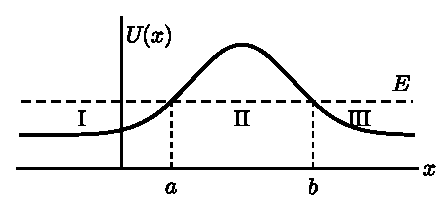
\includegraphics[width=6.5cm]{fig13.pdf}\\[0.3em]{\small 图 13}\end{minipage}\par\nopagebreak

为了不中断后面的计算，我们先来求解下列问题.假定在回点 $x=b$ 右侧（该处的 $U(x)<E$）的准经典波函数呈以下的行波形式：
\begin{equation}
  \psi=\frac{C}{\sqrt{p}}\exp\left[\frac{i}{\hbar}\int_b^x p\,\mathrm{d}x+\frac{1}{4}i\pi\right].
\end{equation}

我们来求 $x<b$ 区域内这个态的波函数.这可和§47中的步骤一样，采用复变量 $x$ 的平面.令
\begin{equation*}
  E-U(x)\approx F_0(x-b),\qquad F_0>0,
\end{equation*}
可把(50.1)式写成
\begin{equation*}
  \psi(x)=\frac{C}{(2mF_0)^{1/4}(x-b)^{1/4}}
  \exp\left\{\frac{i}{\hbar}(2mF_0)^{1/2}\int_b^x\sqrt{x-b}\,\mathrm{d}x+\frac{1}{4}i\pi\right\},
\end{equation*}
沿上半平面的下列半圆自右至左地通过：
\begin{equation*}
  x-b=\rho\mathrm{e}^{i\phi},
\end{equation*}
\begin{equation*}
  i\int_b^x\sqrt{x-b}\,\mathrm{d}x
  =\frac{2}{3}\rho^{3/2}\left(-\sin\frac{3}{2}\phi+i\cos\frac{3}{2}\phi\right),
\end{equation*}
相位 $\phi$ 从 0 变到 $\pi$.$\psi(x)$ 函数的模先是递减，随后增大，到达半圆末端的函数值为
\begin{equation*}
  \psi(x)=\frac{C}{(2mF_0)^{1/4}(b-x)^{1/4}}
  \exp\left\{\frac{1}{\hbar}(2mF_0)^{1/2}\int_x^b\sqrt{b-x}\,\mathrm{d}x+\frac{1}{4}i\pi\right\}.
\end{equation*}
我们就得到下列对应规则\footnote{沿下半平面自右向左通过时，$\psi(x)$ 函数的模先增后减，到达左实轴上（$\phi\to-\pi$）变成一个指数式小量，把它始终加到(50.2)指数式大的项上将是不合理的.在 $\psi(x)$ 为指数式大的区域内，由于准经典近似的不精确性，会丢掉指数式小的修正项.而这个修正项当 $\phi\to-\pi$ 时又能变成指数式大项，因而后者也就会被丢掉.}.
\begin{equation}
\begin{array}{ll}
  x>b\ \text{处} &
  \dfrac{C}{\sqrt{p}}\exp\Big\{\dfrac{i}{\hbar}\int_b^x p\,\mathrm{d}x
  +\dfrac{1}{4}i\pi\Big\}\\[2ex]
  x<b\ \text{处} &
  \dfrac{C}{\sqrt{|p|}}\exp\Big\{\dfrac{1}{\hbar}
  \Big|\int_b^x p\,\mathrm{d}x\Big|\Big\}.
\end{array}
\end{equation}

必须强调，此式预先假定了经典通区内波函数的特殊形状（向右运动的行波），应用时只能从通区过渡到禁区.

现在来计算穿过势垒的透射系数.设粒子自Ⅰ区由左向右射向势垒.则在势垒后面的Ⅲ区内，只能有穿过势垒向右运动的波，此区内的波函数可写成
\begin{equation}
  \psi=\sqrt{\frac{D}{v}}\exp\left(\frac{i}{\hbar}\int_b^x p\,\mathrm{d}x+\frac{1}{4}i\pi\right),
\end{equation}
式中的 $v=p/m$ 是粒子速度，$D$ 是流密度.应用规则(50.2)，可以求出势垒内部Ⅱ区的波函数：
\begin{equation}
\begin{aligned}
  \psi_{II}&=\sqrt{\frac{D}{|v|}}\exp\left(\frac{1}{\hbar}\bigg|\int_x^b p\,\mathrm{d}x\bigg|\right)=\\
  &=\sqrt{\frac{D}{|v|}}\exp\left(\frac{1}{\hbar}\bigg|\int_a^b p\,\mathrm{d}x\bigg|
  -\frac{1}{\hbar}\bigg|\int_a^x p\,\mathrm{d}x\bigg|\right).
\end{aligned}
\end{equation}

最后，应用规则(47.5)，可得势垒前面Ⅰ区的波函数：
\begin{equation*}
  \psi=2\sqrt{\frac{D}{v}}\exp\left(\frac{1}{\hbar}\int_a^b|p|\,\mathrm{d}x\right)
  \cos\left(\frac{1}{\hbar}\int_a^x p\,\mathrm{d}x+\frac{1}{4}\pi\right).
\end{equation*}
如果我们令
\begin{equation}
  D=\exp\left(-\frac{2}{\hbar}\int_a^b|p|\,\mathrm{d}x\right),
\end{equation}
上式变成
\begin{equation*}
\begin{aligned}
  \psi&=\frac{2}{\sqrt{v}}\cos\left(\frac{1}{\hbar}\int_a^x p\,\mathrm{d}x+\frac{1}{4}\pi\right)=\\
  &=\frac{1}{\sqrt{v}}\exp\left(\frac{1}{\hbar}\int_a^x p\,\mathrm{d}x+\frac{1}{4}i\pi\right)+\\
  &\quad+\frac{1}{\sqrt{v}}\exp\left(-\frac{1}{\hbar}\int_a^x p\,\mathrm{d}x-\frac{1}{4}i\pi\right).
\end{aligned}
\end{equation*}
第一项代表射向势垒的波（$x\to-\infty$ 时变成平面波 $\psi=\mathrm{e}^{ipx/\hbar}$），第二项代表反射波，所选的归一化已使入射波具有单位流密度，因此透射波的流密度 $D$ 就等于所求的势垒透射系数.注意此公式只当指数幂很大因而 $D$ 本身很小时才能适用.\footnote{$D$ 为指数式小量，这与Ⅰ区内入射波和反射波的振幅相等这个事实有关；两者之间指数式小的差别在准经典近似中被丢掉.}

前面已经假定了场 $U(x)$ 在整个势垒范围内满足准经典条件（只有在回点的邻区除外）.但在实际上我们常常遇到这样的势垒，它的势能曲线在一侧降落得极快，使得准经典近似无法应用.在这种情况下，(50.5)式 $D$ 中的指数因子仍保持不变，但其前面的系数［在(50.5)式中等于1］有所不同.要算出这个系数，我们必须算出非准经典区内的精确波函数，并据此定出势垒内部的准经典波函数.

\begin{xiti}

\noindent{\heiti 习题1}\quad 求图14所示的势垒的透射系数：$x<0$ 时 $U(x)=0$，$x>0$ 时 $U(x)=U_0-Fx$；只需算出指数因子.

解：简单计算后给出下列结果：
\begin{equation*}
  D\sim\exp\bigg[-\frac{4\sqrt{2m}}{3\hbar F}(U_0-E)^{3/2}\bigg].
\end{equation*}

\par\nopagebreak\noindent\begin{minipage}{\linewidth}\centering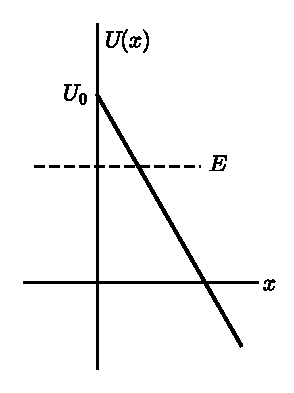
\includegraphics[width=4.5cm]{fig14.pdf}\\[0.3em]{\small 图 14}\end{minipage}\par\nopagebreak

\noindent{\heiti 习题2}\quad 求一粒子（角动量等于零）逸出一球对称势阱的概率，该势阱当 $r<r_0$ 时 $U(r)=-U_0$，$r>r_0$ 时 $U(r)=\dfrac{\alpha}{r}$（图15）.\footnote{这个问题首先由 Г.~Ф.~Гамовым（1928）以及由 R.~W.~Gurney 和 E.~U.~Condon（1929）在关于放射性 $\alpha$ 衰变的理论中讨论过.}

\par\nopagebreak\noindent\begin{minipage}{\linewidth}\centering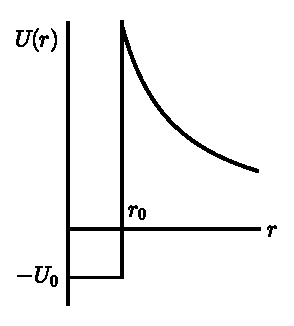
\includegraphics[width=4.5cm]{fig15.pdf}\\[0.3em]{\small 图 15}\end{minipage}\par\nopagebreak

解：球对称问题可以归结为一维问题，因此以前所得的公式可以直接应用.我们有
\begin{equation*}
  w\sim\exp\bigg[-\frac{2}{\hbar}\int_{r_0}^{\alpha/E}
  \sqrt{2m\left(\frac{\alpha}{r}-E\right)}\,\mathrm{d}r\bigg].
\end{equation*}
算出此积分，最后得
\begin{equation*}
  w\sim\exp\bigg\{-\frac{2\alpha}{\hbar}\sqrt{\frac{2m}{E}}
  \bigg[\operatorname{arccos}\sqrt{\frac{Er_0}{\alpha}}
  -\sqrt{\frac{Er_0}{\alpha}\left(1-\frac{Er_0}{\alpha}\right)}\bigg]\bigg\}.
\end{equation*}
在 $r_0\to0$ 的极限情形下，此式变成
\begin{equation*}
  w\sim\exp\bigg\{-\frac{\pi\alpha}{\hbar}\sqrt{\frac{2m}{E}}\bigg\}
  =\exp\bigg\{-\frac{2\pi\alpha}{\hbar v}\bigg\}.
\end{equation*}
这个公式，当指数幂很大即 $\alpha/\hbar v\gg1$ 时可以适用.这个条件和库仑场中的准经典运动条件(49.11)式一致.

\noindent{\heiti 习题3}\quad 设 $U(x)$ 由两个对称的势阱（图16中的Ⅰ和Ⅱ）夹一个势垒所组成.如果该势垒对粒子不可穿透，则其能级对两个势阱相同，相当于粒子在其中一个势阱中运动时所具有的那些能级.势垒的可穿透这一事实，使得以上的每个能级分裂成两个相邻能级，对应于粒子同时在两个势阱中运动时的两种不同状态.试求分裂宽度［假定势场 $U(x)$ 是准经典的］.

\par\nopagebreak\noindent\begin{minipage}{\linewidth}\centering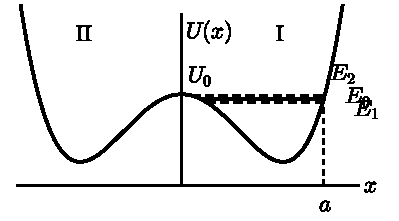
\includegraphics[width=5.5cm]{fig16.pdf}\\[0.3em]{\small 图 16}\end{minipage}\par\nopagebreak

解：略去穿过势垒的概率，$U(x)$ 场中的薛定谔方程的近似解可以采用准经典波函数 $\psi_0(x)$，这个波函数描述在一个势阱中（譬如阱Ⅰ）以某个能量 $E_0$ 运动的粒子，它在该阱两侧指数式衰减；$\psi_0(x)$ 假定是这样归一化的，使得 $\psi_0^2$ 对阱Ⅰ的积分等于1.计入小的透射概率以后，能级 $E_0$ 分裂成 $E_1$ 和 $E_2$ 两能级，对应于这两个能级的正确零级近似波函数，是 $\psi_0(x)$ 和 $\psi_0(-x)$ 的对称和反对称组合：
\setcounter{equation}{0}\renewcommand{\theequation}{\arabic{equation}}%
\begin{equation}
  \psi_1(x)=\frac{1}{\sqrt{2}}\left[\psi_0(x)+\psi_0(-x)\right],\qquad
  \psi_2(x)=\frac{1}{\sqrt{2}}\left[\psi_0(x)-\psi_0(-x)\right].
\end{equation}

阱Ⅰ中，$\psi_0(-x)$ 与 $\psi_0(x)$ 相比小至可略；阱Ⅱ中则反之.故乘积 $\psi_0(x)\psi_0(-x)$ 处处都小至可略.(1)式中的两个函数可这样归一化，使它们的平方值对阱Ⅰ加阱Ⅱ积分后都等于1.

薛定谔方程为
\begin{equation*}
  \psi_0''+\frac{2m}{\hbar^2}(E_0-U)\psi_0=0,\qquad
  \psi_1''+\frac{2m}{\hbar^2}(E_1-U)\psi_1=0,
\end{equation*}
第一式乘以 $\psi_1$ 第二式乘以 $\psi_0$ 后，两式相减，然后对 $\mathrm{d}x$ 从 0 到 $\infty$ 积分.考虑到 $x=0$ 时，$\psi_1=\sqrt{2}\psi_0$ 和 $\psi_1'=0$，以及
\begin{equation*}
  \int_0^{\infty}\psi_0\psi_1\,\mathrm{d}x
  \approx\frac{1}{\sqrt{2}}\int_0^{\infty}\psi_0^2\,\mathrm{d}x
  =\frac{1}{\sqrt{2}},
\end{equation*}
我们得
\begin{equation*}
  E_1-E_0=-\frac{\hbar^2}{m}\psi_0(0)\psi_0'(0).
\end{equation*}
同理，我们发现 $E_2-E_0$ 具有相同的表式，但差一负号，故
\begin{equation*}
  E_2-E_1=\frac{2\hbar^2}{m}\psi_0(0)\psi_0'(0).
\end{equation*}
根据(47.1)式，以及(48.3)式中系数 $C$，我们有
\begin{equation*}
  \psi_0(0)=\sqrt{\frac{\omega}{2\pi v_0}}
  \exp\left(-\frac{1}{\hbar}\int_0^a|p|\,\mathrm{d}x\right),\qquad
  \psi_0'(0)=\frac{mv_0}{\hbar}\psi_0(0),
\end{equation*}
其中的 $v_0=\sqrt{2(U_0-E_0)/m}$.故
\begin{equation*}
  E_2-E_1=\frac{\omega\hbar}{\pi}
  \exp\left(-\frac{1}{\hbar}\int_{-a}^a|p|\,\mathrm{d}x\right).
\end{equation*}
$a$ 是对应于能量 $E_0$ 的回点，见图16.

\noindent{\heiti 习题4}\quad 粒子穿过一抛物势垒 $U(x)=-\dfrac{1}{2}kx^2$，试求透射系数 $D$ 的精确值（假定 $D$ 不是很小）.（E.~C.~Kemble,1935）\footnote{此题之解也可应用到任一势垒 $U(x)$ 顶点附近的透射，只要 $U(x)$ 在极大值附近依赖于 $x$ 的平方.}.

解：不管 $\hbar$ 和 $E$ 的数值如何，在足够大的 $|x|$ 距离处运动是准经典的，该处的
\begin{equation*}
  p=\sqrt{2m\left(E+\frac{1}{2}kx^2\right)}
  \approx x\sqrt{mk}+E\sqrt{\frac{m}{k}}\,\frac{1}{x}.
\end{equation*}
薛定谔方程之解的渐近式为
\begin{equation*}
  \psi=\text{常数}\times\mathrm{e}^{\pm\frac{1}{2}i\xi^2}\xi^{\pm i\varepsilon-1/2},
\end{equation*}
其中引用了下列记号：
\begin{equation*}
  \xi=x\left(\frac{mk}{\hbar^2}\right)^{1/4},\qquad
  \varepsilon=\frac{E}{\hbar}\sqrt{\frac{m}{k}}.
\end{equation*}
我们只对这样的解感兴趣：当 $x\to+\infty$ 时此解只含自左向右运动（已经越过势垒）的波.我们令
\setcounter{equation}{0}%
\begin{equation}
  x\to+\infty\ \text{时},\quad
  \psi=B\mathrm{e}^{i\xi^2/2}\xi^{i\varepsilon-1/2},
\end{equation}
\begin{equation}
  x\to-\infty\ \text{时},\quad
  \psi=\mathrm{e}^{-i\xi^2/2}(-\xi)^{-i\varepsilon-1/2}
  +A\mathrm{e}^{i\xi^2/2}(-\xi)^{i\varepsilon-1/2}.
\end{equation}
(2)式中的第一项代表入射波，第二项为反射波（波的行进方向是它的相位增加方向）.$A$ 和 $B$ 之间的关系可以从以下的事实出发求出，即 $\psi$ 的渐近表式在 $\xi$ 复变量平面上的足够远的整个区域内都是成立的.现在来考察函数(1)沿 $\xi$ 上半平面内半径 $\rho$ 很大的一个半圆周上的变化.
\begin{equation*}
  \xi=\rho\mathrm{e}^{i\phi},\qquad
  i\xi^2=\rho^2(-\sin2\phi+i\cos2\phi).
\end{equation*}
$\phi$ 从 0 变到 $\pi$.绕此半圆的结果，函数(1)变成(2)中的第二项，具有系数
\begin{equation}
  A=B(\mathrm{e}^{i\pi})^{i\varepsilon-1/2}=-iB\mathrm{e}^{-\pi\varepsilon}.
\end{equation}
在路径的 $\left(\frac{1}{2}\pi<\phi<\pi\right)$ 段内，模 $|\mathrm{e}^{i\xi^2/2}|$ 指数式地增大，指数式小量被丢掉\footnote{通过下半平面求 $A$ 是不恰当的，因为在与终端［端点处的 $\psi$ 值由(2)式给出］相联的路段 $\left(-\pi<\phi<-\frac{1}{2}\pi\right)$ 上，$\mathrm{e}^{i\xi^2/2}$ 项与 $\mathrm{e}^{-i\xi^2/2}$ 项相比是一个指数式小量.}.

按(2)中入射波所选的归一化，粒子数守恒条件为
\begin{equation}
  |A|^2+|B|^2=1,
\end{equation}
由(3)和(4)得到所求的透射系数
\begin{equation*}
  D=|B|^2=1/(1+\mathrm{e}^{-2\varepsilon\pi}),
\end{equation*}
此式对任何 $E$ 都成立，如果能量的绝对值很大并且是负的，则得 $D\approx\mathrm{e}^{-2\pi|\varepsilon|}$，与(50.5)式一致.对 $E>0$，量
\begin{equation*}
  R=1-D=1/(1+\mathrm{e}^{2\pi\varepsilon})
\end{equation*}
是势垒之上的反射系数.

\end{xiti}
\renewcommand{\theequation}{\arabic{section}.\arabic{equation}}%

\section{准经典矩阵元的计算}

要直接计算任一物理量 $f$ 对准经典波函数而言的矩阵元，存在着很大的困难.我们假定，所求矩阵元中的那两个跃迁态的能量值并不十分靠近，使得该矩阵元不能化成 $f$ 的傅里叶分量（§48）.困难的产生，在于这样的波函数都呈指数形式（指数幂是一个很大的虚量），被积函数呈现急剧的振荡.

我们来考虑一维的情形［在势场 $U(x)$ 中运动］，为简单计，假定该物理量的算符只是一个坐标函数 $f(x)$.设 $\psi_1$ 和 $\psi_2$ 为对应于粒子能量值 $E_1$ 和 $E_2$（且 $E_2>E_1$，图17）的两个波函数；我们假定 $\psi_1$ 和 $\psi_2$ 都取为实函数.现在要计算下列积分：
\begin{equation}
  f_{12}=\int_{-\infty}^{\infty}\psi_1 f\psi_2\,\mathrm{d}x.
\end{equation}

\par\nopagebreak\noindent\begin{minipage}{\linewidth}\centering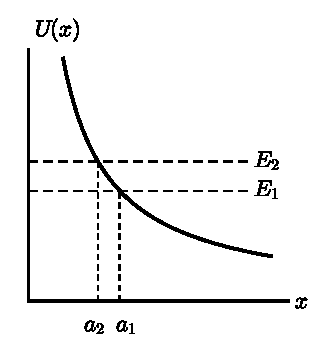
\includegraphics[width=5cm]{fig17.pdf}\\[0.3em]{\small 图 17}\end{minipage}\par\nopagebreak

按(47.5)，在回点 $x=a_1$ 的两侧区域，但不在 $a_1$ 点的紧邻区域内，$\psi_1$ 波函数呈下列形式：
\begin{equation}
  x<a_1,\quad
  \psi_1=\frac{C_1}{2\sqrt{|p_1|}}\exp\left(-\frac{1}{\hbar}
  \bigg|\int_{a_1}^x p_1\,\mathrm{d}x\bigg|\right),
\end{equation}
\begin{equation*}
  x>a_1,\quad
  \psi_1=\frac{C_1}{\sqrt{p_1}}\cos\left(\frac{1}{\hbar}\int_{a_1}^x p_1\,\mathrm{d}x-\frac{1}{4}\pi\right),
\end{equation*}
对 $\psi_2$ 也有同样的式子（下标1改成2）.

可是，如果把波函数的这些渐近式代入(51.1)式中进行积分计算，并不能得到正确的结果.我们将在下面看到，原因在于这个积分是一个指数式的小量，而被积函数本身却并不很小.因此被积函数只要相对地作出很小的改变，它的积分值一般讲来就会有成数量级的变化.这种困难可以用以下的方法加以避免.

我们把 $\psi_2$ 函数表成 $\psi_2=\psi_2^++\psi_2^-$，也就是把余弦函数（在 $x>a_2$ 的区域内）表成两个指数式之和.按照(50.2)式，我们有
\begin{equation}
\begin{aligned}
  x<a_2,\ \psi_2^+&=\frac{-iC_2}{2\sqrt{|p_2|}}\exp\left(\frac{1}{\hbar}
  \bigg|\int_{a_2}^x p_2\,\mathrm{d}x\bigg|\right),\\
  x>a_2,\ \psi_2^+&=\frac{C_2}{2\sqrt{p_2}}\exp\left[\frac{i}{\hbar}\int_{a_2}^x p_2\,\mathrm{d}x
  -\frac{1}{4}i\pi\right];
\end{aligned}
\end{equation}
$\psi_2^-$ 函数是 $\psi_2^+$ 的共轭复函数［$\psi_2^-=(\psi_2^+)^*$］.

积分式(51.1)也被分为两个复共轭积分之和 $f_{12}=f_{12}^++f_{12}^-$，这是我们想要计算的.首先，我们注意到下列积分是收敛的：
\begin{equation*}
  f_{12}^+=\int_{-\infty}^{\infty}\psi_1 f\psi_2^+\,\mathrm{d}x,
\end{equation*}
实际上，尽管 $\psi_2^+$ 函数在 $x<a_2$ 区域内指数式地增长，但是 $\psi_1$ 函数在 $x<a_1$ 区域内按指数形式更快地趋于零（由于在 $x<a_2$ 区域内到处都有 $|p_1|>|p_2|$）.

我们把坐标 $x$ 看作一个复变量，并把积分路线从实轴移到上半平面.当 $x$ 多出一个正的虚增量时，$\psi_1$ 函数（在 $x>a_1$ 区域内）中出现一个递增项，但是 $\psi_2^+$ 函数仍递减得更快，因为在 $x>a_1$ 区域内到处都有 $p_2>p_1$.结果使被积函数衰减.

移动后的积分路线不再通过实轴上的 $x=a_1,a_2$ 两点（这两点附近准经典近似不能适用）.因此在整个积分路线上，我们可以应用 $\psi_1$ 和 $\psi_2^+$ 函数在上半平面中的渐近式，这些表式是
\begin{equation}
\begin{aligned}
  \psi_1&=\frac{C_1}{2\left[2m(U-E_1)\right]^{1/4}}\exp\left(\frac{1}{\hbar}
  \int_{a_1}^x\sqrt{2m(U-E_1)}\,\mathrm{d}x\right),\\
  \psi_2^+&=\frac{-iC_2}{2\left[2m(U-E_2)\right]^{1/4}}\exp\left(-\frac{1}{\hbar}
  \int_{a_2}^x\sqrt{2m(U-E_2)}\,\mathrm{d}x\right),
\end{aligned}
\end{equation}
其中的根号是这样选取的，使得 $x<a_1,a_2$ 时它们在实轴上取正值.

在下列积分式中：
\begin{equation}
\begin{aligned}
  f_{12}^+=\frac{-iC_1C_2}{4\sqrt{2m}}\int\exp\bigg(\frac{1}{\hbar}
  \int_{a_1}^x\sqrt{2m(U-E_1)}\,\mathrm{d}x
  -\frac{1}{\hbar}\int_{a_2}^x\sqrt{2m(U-E_2)}\,\mathrm{d}x\bigg)\times\\
  \times\frac{f(x)\,\mathrm{d}x}{\left[(U-E_1)(U-E_2)\right]^{1/4}},
\end{aligned}
\end{equation}

我们希望改变积分路径，使得指数因子尽可能减小.上式中的指数幂只在 $U(x)=\infty$ 的点具有一个极值（因为 $E_1\neq E_2$ 时，指数幂对 $x$ 的微商在其它点都不等于零）.因此积分路径改变到上半平面内的唯一限制是，该路径必须绕过 $U(x)$ 函数的奇点；按照线性微分方程的一般理论，这些奇点也就是 $\psi(x)$ 波函数的奇点.积分路径的具体选择依赖于 $U(x)$ 场的实际形状.如果 $U(x)$ 函数在上半平面只有 $x=x_0$ 的一个奇点，那么该积分可取图18所示的那种路径进行.这个奇点的邻域在该积分中占有重要地位，使得欲求的矩阵元 $f_{12}=2\,\mathrm{Re}\,f_{12}^+$ 实际上和下列指数幂很小的表式成正比：

\par\nopagebreak\noindent\begin{minipage}{\linewidth}\centering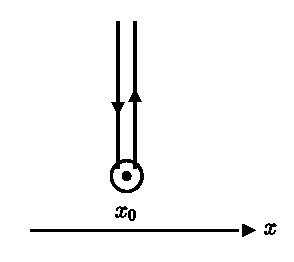
\includegraphics[width=4.5cm]{fig18.pdf}\\[0.3em]{\small 图 18}\end{minipage}\par\nopagebreak

\begin{equation}
\begin{aligned}
  &f_{12}\sim\exp\bigg(-\frac{1}{\hbar}\,\mathrm{Im}\bigg[\int^{x_0}\sqrt{2m(E_2-U)}\,\mathrm{d}x
  -\int^{x_0}\sqrt{2m(E_1-U)}\,\mathrm{d}x\bigg]\bigg)\\
  &\qquad\qquad\qquad\qquad\qquad\qquad
  (\text{Л. Д. Ландау},1932)\text{\footnotemark}.
\end{aligned}
\end{equation}
\footnotetext{在(51.5)和(51.6)式的推导中，我们把波函数改成了它们的渐近式，由于采用了图18所示的积分路径，这个积分式的数量级就决定于被积函数的数量级；因此被积函数的很小改变对积分值不会有很大影响.}

这两个积分式的积分下限可取经典通区中的任意点；很明显，积分式的虚部不依赖于这两个点的具体选择方式.如果 $U(x)$ 函数在上半平面具有好几个奇点，则(51.6)式中应该取这样的 $x_0$ 点，使得式中的指数幂具有最小的绝对值\footnote{我们已经假定了 $f(x)$ 本身并没有奇点.还要注意，估计矩阵元数量级的(51.6)式，是在指数式前面的系数具有“正常”数量级的前提下写出的.当然，可能存在一些特殊情况使得这一系数变成“非正常地”小.一个最简单的例子是 $f(x)=$ 常数，这时由于波函数的正交性使得矩阵元成为零.这种情况在(51.6)式上看不出来.}.

当两个能量 $E_1$ 和 $E_2$ 相差不多的时候，公式(51.6)可以简化.这时，根据§48的结果，矩阵元简化为经典量 $f[x(t)]$ 对时间的傅里叶积分.令 $E_{2,1}=E\pm\dfrac{\hbar\omega_{21}}{2}$ 并按 $\hbar\omega_{21}$ 展开，得
\begin{equation*}
  f_{12}\sim\exp\bigg(-\omega_{21}\,\mathrm{Im}\int^{x_0}\sqrt{\frac{m}{2(E-U)}}\,\mathrm{d}x\bigg)
  =\exp\big(-\omega_{21}\,\mathrm{Im}\,\tau\big).\tag{51.6a}
\end{equation*}
下列这个量
\begin{equation*}
  \tau=\int^{x_0}\sqrt{\frac{m}{2(E-U)}}\,\mathrm{d}x
  =\int^{x_0}\frac{\mathrm{d}x}{v(x)}
\end{equation*}
可以看成是复时间，即在 $x$ 的复平面上粒子到 $x_0$ 点所用的时间（而 $v(x)=\sqrt{2(E-U(x))/m}$ 是相应的“复速度”）.不难看出，(51.6a)实际上给出的是，在条件 $\mathrm{Im}\,\tau\gg1$ 之下 $f[x(t)]$ 的复傅里叶展开的渐近式.

用同一方法，可计算有心力场运动中的准经典矩阵元.但是 $U(r)$ 现在必须理解成为有效势能（势能与离心能之和），对 $l$ 值不同的态而言，有效势能是不同的.为了在以后的问题中进一步应用这个方法起见，我们把两个不同态中的有效势能写成 $U_1(r)$ 和 $U_2(r)$ 的一般形式.此时，(51.5)被积函数中的指数幂不但在 $U_1(r)$ 或 $U_2(r)$ 等于无穷大那些点具有极值，并且还在满足下列方程那些点具有极值：
\begin{equation}
  U_2(r)-U_1(r)=E_2-E_1.
\end{equation}
因此在以下公式内
\begin{equation}
\begin{aligned}
  f_{12}\sim\exp\bigg(-\frac{1}{\hbar}\,\mathrm{Im}\bigg[\int^{r_0}\sqrt{2m(E_2-U_2)}\,\mathrm{d}r
  -\int^{r_0}\sqrt{2m(E_1-U_1)}\,\mathrm{d}r\bigg]\bigg),
\end{aligned}
\end{equation}
$r_0$ 的可能值中不只包括 $U_1(r)$ 和 $U_2(r)$ 的各个奇点，并且还包括(51.7)式的各个根.

有心力场情形还有一个不同之处，在(51.1)式中它对 $\mathrm{d}r$ 的积分是从 0（不是从 $-\infty$）到 $\infty$ 的：
\begin{equation*}
  f_{12}=\int_0^{\infty}\chi_1 f\chi_2\,\mathrm{d}r.
\end{equation*}
这里有两种情况必须区别，如果被积函数是 $r$ 的偶函数，那么这个积分式可以在形式上延伸到从 $-\infty$ 到 $+\infty$ 的整个区间，从而和以前的情形毫无区别.如果 $U_1(r)$ 和 $U_2(r)$ 都是 $r$ 的偶函数［$U(-r)=U(r)$］，上述情况就有可能发生.此时的波函数 $\chi_1(r)$ 和 $\chi_2(r)$ 或者是偶函数或者是奇函数\footnote{$U(r)$ 为偶函数时，径向波函数 $R(r)$ 的奇偶决定于 $l$ 的奇偶.这可从 $r$ 很小时的 $R(r)$ 看出来（此时有 $R\sim r^l$）.}（见§21），假若 $f(r)$ 函数也是偶的或奇的，乘积 $\chi_1 f\chi_2$ 就有可能是偶函数.

另一方面，如果被积函数不是偶函数［如果 $U(r)$ 不是偶函数，就有这种情况］，那么积分路径的起点就不能从 $r=0$ 点移开，而且 $r_0=0$ 点的值就应包含在(51.8)式的 $r_0$ 的各种可能值中.

\begin{xiti}

\noindent{\heiti 习题1}\quad 计算 $U=U_0\mathrm{e}^{-\alpha x}$ 场中的准经典矩阵元（只算指数因子）.

解：$U(x)$ 只有 $x\to-\infty$ 时变成无穷大.相应地可令(51.6)中的 $x_0=-\infty$.这个积分可以延伸到 $x=+\infty$.方括号内每一项积分时，都在其下限 $-\infty$ 处发散.因此我们先计算从 $-x$ 到 $+\infty$ 的积分，然后再取极限 $x\to\infty$.结果得
\begin{equation*}
  f_{12}\sim\exp\bigg[-\frac{\pi m}{\alpha\hbar}(v_2-v_1)\bigg],
\end{equation*}
其中的 $v_1=\sqrt{2E_1/m}$，$v_2=\sqrt{2E_2/m}$ 为无穷远处（$x\to\infty$）的粒子速度，该处的运动是自由运动.

\noindent{\heiti 习题2}\quad 与题1相同，但在库仑场 $U=\alpha/r$ 中，求 $l=0$ 的两个态间的准经典跃迁矩阵元.

解：$U(r)$ 函数的唯一奇点是 $r=0$.相应的积分式已在§50题2中算过.按(51.8)式，结果得
\begin{equation*}
  f_{12}\sim\exp\bigg[\frac{\pi\alpha}{\hbar}
  \left(\frac{1}{v_2}-\frac{1}{v_1}\right)\bigg].
\end{equation*}

\noindent{\heiti 习题3}\quad 同第一题，求非谐振子的跃迁矩阵元，其势能为
\begin{equation*}
  U(x)=\frac{m\omega^2}{2}x^2+\beta x^4
\end{equation*}
在下列条件下计算：
\setcounter{equation}{0}\renewcommand{\theequation}{\arabic{equation}}%
\begin{equation}
  \hbar\omega\ll E_1,\qquad E_2\ll\frac{m^2\omega^4}{\beta}.
\end{equation}

解：对正文中所讲有限运动的推广表明，公式(51.6)仍旧成立，应当选取两个点 $x\to\pm\infty$ 作为 $x_0$，这两个点都带来一个数量级的贡献.我们有
\begin{equation*}
  f_{12}\sim\exp\bigg(-\frac{1}{\hbar}\bigg[\int_{a_2}^{-\infty}\sqrt{2m(U-E_2)}\,\mathrm{d}x
  -\int_{a_1}^{-\infty}\sqrt{2m(U-E_1)}\,\mathrm{d}x\bigg]\bigg).
\end{equation*}
在(1)式条件之下，给出主要贡献的区域是
\begin{equation}
  \sqrt{\frac{E_1}{m\omega^2}},\ \sqrt{\frac{E_2}{m\omega^2}}\ll|x|
  \ll\sqrt{\frac{m\omega^2}{\beta}},
\end{equation}
其中
\begin{equation*}
  \frac{m\omega^2}{2}x^2\gg E_1,\,E_2,\,\beta x^4.
\end{equation*}
将指数展开为 $(E_{1,2}/U)$ 的幂级数（这时零次项互相抵消）并忽略 $\beta x^4$，得
\begin{equation*}
  f_{12}\sim\exp\bigg(-\frac{E_2}{\hbar\omega}\int\frac{\mathrm{d}|x|}{|x|}
  +\frac{E_1}{\hbar\omega}\int\frac{\mathrm{d}|x|}{|x|}\bigg).
\end{equation*}
在区间(2)中对数发散的积分应予舍去，即在上限 $x\sim\sqrt{(m\omega^2)/\beta}$ 时和在下限 $x\sim a_2\sim\sqrt{E_2/(m\omega^2)}$ 及 $x\sim a_1\sim\sqrt{E_1/(m\omega^2)}$ 时，结果得
\begin{equation*}
  f_{12}\sim\exp\bigg(-\frac{E_2}{2\hbar\omega}\ln\frac{m^2\omega^4}{\beta E_2}
  +\frac{E_1}{2\hbar\omega}\ln\frac{m^2\omega^4}{\beta E_1}\bigg).
\end{equation*}
引入态的数目，
\begin{equation*}
  n_1\approx E_1/\hbar\omega,\qquad n_2\approx E_2/\hbar\omega,
\end{equation*}
可将答案写成
\begin{equation*}
  f_{12}\sim\frac{n_2^{n_2/2}}{n_1^{n_1/2}}
  \bigg(\frac{\beta\hbar}{m\omega^3}\bigg)^{(n_2-n_1)/2}.
\end{equation*}
既然在解题过程中存在较大的 $x$ 值，这个解答在 $f(x)$ 不过快地趋近无穷大时是成立的.如果将 $f(x)$ 展开成为多项式，那么它的幂次应该比 $(n_2-n_1)$ 小.

\end{xiti}
\renewcommand{\theequation}{\arabic{section}.\arabic{equation}}%

\section{准经典情形下的跃迁概率}

势垒贯穿是经典力学中完全不可能实现的一个例子.准经典情形下这个过程的概率是一个指数式的小量.它的有关指数幂可用下法确定.

考虑任一系统从一态到另一态的跃迁，我们解出相应的经典运动方程，求出其跃迁“轨道”；但是根据经典力学中并不出现这种过程的事实，这必然是复数解.例如，我们发现，系统从一态形式上跃迁到另一态的那个“跃迁点”$q_0$ 一般讲来是一个复数点；该点的位置由经典守恒律所确定.然后我们来计算系统的作用量 $S_1(q_1,q_0)+S_2(q_0,q_2)$，该系统在第一个态中从某个初位置 $q_1$ 出发运动到“跃迁点”$q_0$，再在第二个态中从 $q_0$ 点出发到达最后的 $q_2$ 位置.所求的这一过程的概率由下式给出
\begin{equation}
  w\sim\exp\bigg\{-\frac{2}{\hbar}\,\mathrm{Im}\big[S_1(q_1,q_0)+S_2(q_0,q_2)\big]\bigg\}.
\end{equation}

如果“跃迁点”的位置不是唯一的，则应从中选取这样的点，使得(52.1)式中的指数幂具有最小的绝对值［当然，这个绝对值还应足够的大，使得(52.1)式仍能成立］.\footnote{如果该系统的势能本身具有奇点，那么这些奇点也应算入 $q_0$ 的可能值中.}

(52.1)式是和§51中计算准经典矩阵元时导出的规则一致的，但应指出，采用矩阵元的平方去计算跃迁概率中指数前的系数，将是不正确的.

基于(52.1)式的复经典轨道法是一个普遍方法，它可适用于具有任意多自由度的系统中的跃迁（Л. Д. Ландау,1932）.如果跃迁点是实数但位于经典禁区内，则（在一维运动的简单情形下）(52.1)式与势垒贯穿的概率式(50.5)相同.

\subsection*{垒顶之上的反射}

让我们把(52.1)式应用于垒顶反射的一维问题，所谓垒顶之上的反射，就是指粒子能量超过势垒高度时发生的反射.在这种情形下，$q_0$ 就取粒子运动反向点（“回点”）$x_0$ 的复坐标，也就是方程 $U(x)=E$ 的复根.我们来看一下，怎样能更精确地算出包括指数前系数在内的反射系数.

我们必须（像§50那样）再一次建立势垒远右侧的波函数（透射波）与远左侧的波函数（入射和反射波）间的关系.采用§47和§50中类似的方法，把 $\psi$ 看作复变量 $x$ 的函数，不难做到这一点.

把透射波写成下列形式
\begin{equation*}
  \psi_+=\frac{1}{\sqrt{p}}\exp\left(\frac{i}{\hbar}\int_{x_1}^x p\,\mathrm{d}x\right),
\end{equation*}
式中的 $x_1$ 为实轴上的任一点，我们来追究它沿上半平面中曲线 $C$ 的变化，$C$ 围绕（在足够远处）回点 $x_0$（图19）；这条曲线的整个最后部分必须位于很远的左区，使得入射波的近似（准经典）波函数中的误差远小于欲求的小量 $\psi_-$.绕过 $x_0$ 点致使 $\sqrt{E-U(x)}$ 改变符号，回到实轴后 $\psi_+$ 函数就变成向左传播的反射波 $\psi_-$\footnote{如绕 $x_0$ 点下面的曲线（例如，简单地沿实轴），$\psi_+$ 函数就转变成入射波.}.由于入射波和透射波的振幅可以看作是相等的，所求的反射系数 $R$ 就简单地等于 $\psi_-$ 和 $\psi_+$ 的模量平方之比：

\par\nopagebreak\noindent\begin{minipage}{\linewidth}\centering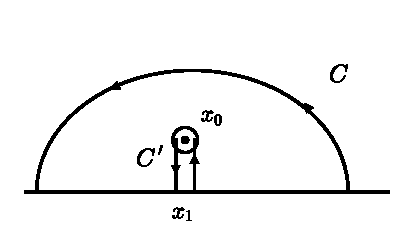
\includegraphics[width=6cm]{fig19.pdf}\\[0.3em]{\small 图 19}\end{minipage}\par\nopagebreak

\begin{equation}
  R=\bigg|\frac{\psi_-}{\psi_+}\bigg|^2
  =\exp\left(-\frac{2}{\hbar}\,\mathrm{Im}\int_C p\,\mathrm{d}x\right).
\end{equation}
导出此式后，指数幂的积分路线就可以任意变形；如果变换到图19所示的 $C'$ 曲线，则上式积分化成从 $x_1$ 到 $x_0$ 的积分的两倍，我们得\footnote{此处给出的证明出自朗道（1961）.}
\begin{equation}
  R=\exp\bigg[\frac{-4}{\hbar}\sigma(x_1,x_0)\bigg],\qquad
  \sigma(x_1,x_0)=\mathrm{Im}\int_{x_1}^{x_0}p(x)\,\mathrm{d}x.
\end{equation}

由于 $p(x)$ 在整个实轴上都是实量，$x_1$ 点的选法无关紧要.\footnote{在某些情况下，值得注意的不仅是入射波和反射波的振幅关系，还有它们的相位关系.这一关系是§25中所述的系数 $\alpha$ 和 $\beta$ 所反映的反射波的振幅所决定的.通过上面的讨论不难看出，从左边射来的波的反射振幅是
\begin{equation*}
  \left(-\frac{\beta^*}{\alpha^*}\right)
  =-i\exp\bigg[\frac{2i}{\hbar}\bigg(\int_{x_1}^{x_0}p\,\mathrm{d}x+p_1x_1\bigg)\bigg],
  \qquad x_1\to-\infty.
\end{equation*}
式中的因子 $(-i)$ 就与通过回点时指数前的系数的相位变化有关.}注意(52.3)中指数前的系数为1（В.~Л.~Покровский, С.~К.~Саввин, Ф.~Р.~Улинич,1958）.\footnote{正文中此结果的推导是由朗道作出的.}

如前所述，在 $x_0$ 的所有可能值中，我们应选这样一个值，使得(52.3)式的指数幂具有最小的绝对值（并且此值必须远大于1）\footnote{当然，我们只考虑 $\sigma>0$ 的 $x_0$ 点，即位于上半平面的 $x_0$ 点.}.这还暗示着，如果势能 $U(x)$ 本身在上半平面具有奇点，对这些点而言，积分 $\sigma(x_1,x_0)$ 具有较大的值\footnote{注意这时图19中的积分路径 $C$ 应该从函数 $U(x)$ 的奇点下方通过.}；否则指数幂将由这些奇点之一来确定，而指数前的系数将不会像(52.3)中那样等于1.如果 $U(x)$ 随着能量 $E$ 的增大在上半平面某处变成无穷大的话，这个条件肯定无法满足：此时满足 $U=E$ 的 $x_0$ 点在趋于极限时十分接近于满足 $U=\infty$ 的 $x_\infty$ 点，因而这两个点对反射系数作出的贡献大小差不多［积分 $\sigma(x_\infty,x_0)\sim1$］，公式(52.3)不再成立.在极限情形下，当 $E$ 大到使得积分值远小于1时，微扰论开始适用（见题2）\footnote{中间情形曾由 В.~Л.~Покровский 和 И.~М.~Халатников 研究过（ЖЭТФ, 40, 1713, 1961）.}.

\begin{xiti}

\noindent{\heiti 习题1}\quad 采用精确到指数因子的准经典近似，求一氘核和一重核（当作有库仑场的固定力心）碰撞时氘核的衰变概率（Е. М. Лифшиц,1939）.

解：对反应概率的主要贡献来自零轨道角动量的碰撞，准经典近似中这就是对头撞，粒子的运动变成一维运动.

令 $E$ 为氘核能量，以 $\epsilon$ 为单位，$\epsilon$ 是氘核的质子和中子的结合能；$E_n$ 和 $E_p$ 为所释放中子和质子的能量，同样以 $\epsilon$ 为单位.我们还采用无量纲坐标 $q=\epsilon r/Ze^2$（$Ze$ 是重核的电荷），并用 $q_0$ 代表 $q$ 在“跃迁点”的值（一般是复值），亦即氘核“衰变时刻”的值.我们可写出
\setcounter{equation}{0}\renewcommand{\theequation}{\arabic{equation}}%
\begin{equation}
  E_n=\frac{1}{2}v_n^2,\qquad
  E_p=\frac{1}{2}v_p^2+\frac{1}{q_0},\qquad
  E=v_d^2+\frac{1}{q_0},
\end{equation}
其中 $v_n$，$v_p$ 和 $v_d$ 是衰变时刻各粒子的速度，以 $\sqrt{\epsilon/m}$ 为单位，$m$ 是核子质量；$v_n$ 是实量并与释出中子的速度相等，但 $v_p$ 和 $v_d$ 都是复量.由跃迁点处的能量和动量守恒条件给出
\begin{equation}
  E_p+E_n=E-1,\qquad v_p+v_n=2v_d.
\end{equation}
故有
\begin{equation*}
  v_p=2i+v_n,\qquad v_d=i+v_n,\qquad
  \frac{1}{q_0}=E+1-v_n^2-2iv_n.
\end{equation*}
跃迁前系统的作用量相当于氘在核场中直到衰变点为止的运动；它的虚部为
\begin{equation}
\begin{aligned}
  \mathrm{Im}\,S_1&=Ze^2\sqrt{\frac{m}{\epsilon}}\,
  \mathrm{Im}\int_{\infty}^{q_0}\sqrt{4\left(E-\frac{1}{q}\right)}\,\mathrm{d}q=\\
  &=Ze^2\sqrt{\frac{m}{\epsilon}}\,
  \mathrm{Im}\bigg\{2q_0v_d-\frac{2}{\sqrt{E}}\cosh^{-1}\sqrt{q_0E}\bigg\}.
\end{aligned}
\end{equation}
跃迁后，作用量相当于中子和质子离开衰变点的运动：
\begin{equation}
\begin{aligned}
  \mathrm{Im}\,S_2&=Ze^2\sqrt{\frac{m}{\epsilon}}\,
  \mathrm{Im}\bigg\{\int_{q_0}^{\infty}v_n\,\mathrm{d}q
  +\int_{q_0}^{\infty}\sqrt{2\left(E_p-\frac{1}{q}\right)}\,\mathrm{d}q\bigg\}=\\
  &=Ze^2\sqrt{\frac{m}{\epsilon}}\,
  \mathrm{Im}\bigg\{-v_nq_0-v_pq_0
  +\sqrt{\frac{2}{E_p}}\operatorname{arcosh}\sqrt{q_0E_p}\bigg\}.
\end{aligned}
\end{equation}
据(52.1)，此过程的概率为
\begin{equation}
  w\sim\exp\bigg\{-\frac{2Ze^2}{\hbar}\sqrt{\frac{m}{\epsilon}}\,
  \mathrm{Im}\bigg[\sqrt{\frac{2}{E_p}}\operatorname{arcosh}\sqrt{q_0E_p}
  -\frac{2}{\sqrt{E}}\operatorname{arcosh}\sqrt{q_0E}\bigg]\bigg\}.
\end{equation}
与两个反双曲余弦函数来自(4)和(3)式的事实相一致，它们的虚部必须分别与 $\mathrm{Im}\,v_p$ 和 $\mathrm{Im}\,v_d$ 具有相同的符号，后两者的符号在(2)式之解中已经这样选定：使得 $\mathrm{Im}(S_1+S_2)>0$.

由于 $w$ 与 $E_n$ 成指数依赖关系，衰变（具有任意的 $E_n$ 和 $E_p=E-1-E_n$ 值）的总概率由指数幂（作为 $E$ 的函数）的最小绝对值给出.分析表明，此事发生在 $E_n\to0$ 时.此时有 $q_0=1/(E+1)$，从(5)式得
\begin{equation*}
  w\sim\exp\bigg\{-\frac{2Ze^2}{\hbar}\sqrt{\frac{m}{\epsilon}}
  \bigg[\sqrt{\frac{2}{E-1}}\operatorname{arccos}\sqrt{\frac{E-1}{E+1}}
  -\frac{2}{\sqrt{E}}\operatorname{arccos}\sqrt{\frac{E}{E+1}}\bigg]\bigg\}.
\end{equation*}
这个公式的成立条件是指数幂必须远大于1.

对 $E_n$ 的非零值算出作用量 $S=S_1+S_2$ 的虚部后，我们可以求出所释放粒子的能量分布.在邻近 $E_n=0$ 处，我们有\footnote{$E_n=0$ 时，函数 $\mathrm{Im}\,S(E_n)$ 有一个尖点，从尖点出发不管对正的和负的 $E_n$（负值对应于中子被重核俘获），函数值都增长.}
\begin{equation*}
  \mathrm{Im}\,S(E_n)-\mathrm{Im}\,S(0)\approx E_n
  \bigg(\frac{\mathrm{d}\,\mathrm{Im}\,S}{\mathrm{d}E_n}\bigg)_{E_n=0}.
\end{equation*}
计算导数后给出
\begin{equation*}
\begin{aligned}
  \frac{\mathrm{d}w}{\mathrm{d}E_n}\sim\exp\bigg\{-\frac{2Ze^2}{\hbar}\sqrt{\frac{m}{\epsilon}}\,
  E_n\bigg[\frac{3-E}{(E-1)(E+1)^2}+\\
  +\frac{1}{\sqrt{2(E-1)^3}}\operatorname{arccos}\sqrt{\frac{E-1}{E+1}}\bigg]\bigg\}.
\end{aligned}
\end{equation*}

\noindent{\heiti 习题2}\quad 如粒子能量满足微扰论条件，求垒顶之上的反射系数.

解：采用(43.1)式，初态和末态波函数是沿相反方向行进的两个平面波，分别按单位流密度归一化和按动量除以 $2\pi\hbar$ 的 $\delta$ 函数归一化，式中的 $\mathrm{d}\nu=\mathrm{d}p'/2\pi\hbar$，而 $p'$ 是反射后动量，算出对 $p'$ 的积分（计及 $\delta$ 函数）后得
\setcounter{equation}{0}%
\begin{equation}
  R=\frac{m^2}{\hbar^2p^2}\bigg|\int_{-\infty}^{\infty}U(x)\mathrm{e}^{2ipx/\hbar}\,\mathrm{d}x\bigg|^2.
\end{equation}
如果微扰论的适用条件得到满足，此式即成立，这个条件为 $Ua/\hbar v\ll1$，$a$ 为势垒宽度（见§45附注3），同时有 $pa/\hbar\lesssim1$.后一条件保证了 $R(p)$ 函数的非指数性：不然的话，(1)式的成立问题尚需作进一步的研究.

\noindent{\heiti 习题3}\quad 当 $U(x)$ 函数在 $x=x_0$ 处具有一个斜率间断点时，试求在准经典势垒垒顶之上的反射系数.

解：如果 $U(x)$ 函数对实的 $x$ 值具有某种奇点，则反射系数主要由该点附近的场所决定，并可用微扰论形式地加以计算，并不要求微扰论对所有的 $x$ 都成立；准经典条件的满足已经足够.我们就得到题2的(1)式，唯一差别是入射粒子的动量必须改成 $p(x)$ 在奇点处的值.

目前情形下我们取斜率间断点为 $x=0$ 点，因此在这点附近有
\begin{equation*}
  x>0\ \text{时}\ U=-F_1x;\qquad
  x<0\ \text{时}\ U=-F_2x.
\end{equation*}
$F_1$ 不同于 $F_2$.对 $x$ 进行积分时，可在被积函数中引进一个阻尼因子 $\mathrm{e}^{\pm\lambda x}$，积分做出后再令 $\lambda\to0$.结果为
\begin{equation*}
  R=\frac{m^2\hbar^2}{16p_0^6}(F_2-F_1)^2,
\end{equation*}
式中的 $p_0=p(0)$.

\end{xiti}
\renewcommand{\theequation}{\arabic{section}.\arabic{equation}}%

\section{浸渐微扰作用下的跃迁}

我们在§41中已经提到过，在微扰随时间的变化十分缓慢的极限情形下，系统自一态到另一态的跃迁概率趋于零.现在来定量地研究这个问题，算出在缓变（浸渐）微扰作用下的跃迁概率（А. М. Дыхне,1961）.

设系统的哈密顿量为时间的缓变函数，当 $t\to\pm\infty$ 时趋向一定的极限.并设 $\psi_n(q,t)$ 和 $E_n(t)$ 是由薛定谔方程 $\hat{H}(t)\psi_n=E_n\psi_n$ 解出的本征函数和能量本征值（依赖于时间参量）；由于 $\hat{H}$ 的时间变化具有浸渐性，$E_n$ 和 $\psi_n$ 的时间变化也是缓慢的.我们面临的问题是，如果 $t\to-\infty$ 时该系统处于 $\psi_1$ 态，求 $t\to+\infty$ 时系统处于某一 $\psi_2$ 态的概率 $w_{12}$.

微扰的缓变性意味着“跃迁过程”具有很长的持续时间，因而作用量的改变（由积分式 $-\int E(t)\,\mathrm{d}t$ 给出）很大.在这个意义上所设问题具有准经典性，所求的概率主要由下列 $t=t_0$ 值确定：
\begin{equation}
  E_1(t_0)=E_2(t_0),
\end{equation}
$t_0$ 相当于经典力学中的“跃迁时刻”（参考§52）；实际上，这样的跃迁在经典力学中当然是不可能的，它表现于方程式(53.1)具有复根.与此有关，就有必要研究 $t$ 为复参量时在 $t=t_0$ 点的邻域内薛定谔方程之解所具有的特性，在 $t_0$ 点处两个能量本征值变成相等.

我们将看到，在该点附近本征函数 $\psi_1,\psi_2$ 将随 $t$ 强烈变化.为了求出其关系，我们先令 $\psi_1,\psi_2$ 的线性组合为 $\varphi_1,\varphi_2$，并满足下列条件：
\begin{equation}
  \int\varphi_1^2\,\mathrm{d}q=\int\varphi_2^2\,\mathrm{d}q=0,\qquad
  \int\varphi_1\varphi_2\,\mathrm{d}q=1.
\end{equation}
只要适当选择复组合系数（$t$ 的函数），总能做到这一点.$\varphi_1$ 和 $\varphi_2$ 在 $t=t_0$ 处没有奇点.

现在把本征函数写成下列线性组合形式：
\begin{equation}
  \psi=a_1\varphi_1+a_2\varphi_2.
\end{equation}
要注意的是，当“时间”$t$ 为复变量时，由于势能 $U(t)\neq U(t)^*$，$\hat{H}(t)$ 算符［呈(17.4)形式］仍等于它的转置算符（$\hat{H}=\tilde{\hat{H}}$）但不再厄米（$\hat{H}\neq\hat{H}^{\dagger}$）.

把(53.3)式代入薛定谔方程，对该式左乘 $\varphi_1$ 或 $\varphi_2$，然后对 $\mathrm{d}q$ 积分.引入下列记号：
\begin{equation}
  H_{ik}(t)=\int\varphi_i\hat{H}\varphi_k\,\mathrm{d}q,
\end{equation}
考虑到哈密顿量的上述性质我们有 $H_{12}=H_{21}$，结果得下列方程组：
\begin{equation}
\begin{aligned}
  H_{11}a_1+H_{12}a_2=Ea_2,\\
  H_{12}a_1+H_{22}a_2=Ea_1.
\end{aligned}
\end{equation}

这个方程组有非零解的条件为 $(H_{12}-E)^2=H_{11}H_{22}$，此式之根给出了能量本征值：
\begin{equation}
  E=H_{12}\pm\sqrt{H_{11}H_{22}}.
\end{equation}

把它代入(53.5)式中，得
\begin{equation}
  \frac{a_2}{a_1}=\pm\sqrt{\frac{H_{11}}{H_{22}}}.
\end{equation}

由(53.6)式可知，为使在 $t=t_0$ 点两个本征值相等，其中的 $H_{11}$ 或 $H_{22}$ 在该点应等于零；我们假定它是 $H_{11}$.在正则点，一个函数一般讲来随 $t-t_0$ 而趋于零，因此有
\begin{equation}
  E(t)-E(t_0)=\pm\ \text{常数}\times\sqrt{t-t_0},
\end{equation}
即 $E(t)$ 在 $t=t_0$ 处具有支点.我们还有 $a_2\sim\sqrt{t-t_0}$，故在 $t=t_0$ 点只有一个本征函数 $\varphi_1$.

现在我们看到，所设问题在形式上完全类似于§52中讨论过的垒顶反射问题.我们有“对时间为准经典的”$\psi(t)$ 波函数，代替了§52中对坐标为准经典的函数，希望求出 $t\to+\infty$ 时波函数中的 $c_2\psi_2\mathrm{e}^{-iE_2t/\hbar}$ 项，而当 $t\to-\infty$ 时波函数为 $\Psi(t)=\psi_1\mathrm{e}^{-iE_1t/\hbar}$.这类似于用 $x\to+\infty$ 的透射波求出 $x\to-\infty$ 的反射波问题.欲求的跃迁概率为 $w_{21}=|c_2|^2$.作用量 $S=-\int E(t)\,\mathrm{d}t$ 是由具有复支点的 $E(t)$ 函数的时间积分给出［正如积分 $\int p\,\mathrm{d}x$ 中的 $p(x)$ 函数具有复支点那样］，因此，所考虑的问题，可以通过 $t$ 复平面上从很大负值到很大正值的一个积分回路加以解决，正如§52中对 $x$ 复平面所作的那样，我们不在这里重复这种推导.

\emergencystretch=5em%
我们假定实轴上有 $E_2>E_1$.此时回路必须位于复变量 $t$ 的上半平面（该处的比值 $\mathrm{e}^{-iE_2t/\hbar}/\mathrm{e}^{-iE_1t/\hbar}$ 是增长的）.结果得下列公式［类似于(52.2)式］
\begin{equation}
  w_{21}=\exp\left(\frac{2}{\hbar}\,\mathrm{Im}\int_{C'}E(t)\,\mathrm{d}t\right),
\end{equation}
\emergencystretch=0pt%
其中的积分沿图19所示的回路（自左向右）进行.

在支点之左的回路上有 $E=E_1$，支点之右的回路上有 $E=E_2$.因此可把(53.9)写成
\begin{equation}
  w_{21}=\exp\bigg(-2\,\mathrm{Im}\int_{t_1}^{t_0}\omega_{21}(t)\,\mathrm{d}t\bigg),
\end{equation}
其中的 $\omega_{21}=(E_2-E_1)/\hbar$，$t_1$ 为实轴 $t$ 上的任一点；$t_0$ 点应选(53.1)式的一个复根，此根位于上半平面内，并使(53.10)式中的指数幂具有最小的绝对值\footnote{$t_0$ 的可能值中尚须包含能使 $E(t)$ 成为无穷大之点；对这些点而言(53.9)式指数前的系数不等于1.}.除了以上自 1 态直接跃迁到 2 态以外，还可能有通过几个中间态的“跃迁方式”；其概率也可用类似的公式表出.例如按 $1\to3\to2$ 的“方式”进行跃迁时，(53.10)式中的积分应改成以下两个积分之和
\begin{equation*}
  \int^{t_0^{(31)}}\omega_{31}(t)\,\mathrm{d}t
  +\int^{t_0^{(23)}}\omega_{23}(t)\,\mathrm{d}t,
\end{equation*}
式中的两个积分上限分别为 $E_1(t),E_3(t)$ 以及 $E_2(t),E_3(t)$ 的两个“交点”.以上的积分式，是采用同时围绕这两个复交点的一个回路后得出的.\footnote{连续谱的中间态问题需另行考虑.}

\begin{xiti}

\noindent{\heiti 习题}\quad 确定服从下列方程
\setcounter{equation}{0}\renewcommand{\theequation}{\arabic{equation}}%
\begin{equation}
  \frac{\mathrm{d}^2x}{\mathrm{d}t^2}+\omega^2(t)x=0
\end{equation}
的经典振子，当其频率 $\omega(t)$ 由 $t\to-\infty$ 时的 $\omega_1$ 到 $t\to+\infty$ 时的 $\omega_2$ 作缓慢变化时，其浸渐不变量的变化（А. М. Дыхне,1960）.

解：方程(1)是由薛定谔方程经过下列变换而来：
\begin{equation*}
  \psi\to x,\quad x\to t;\qquad
  p(x)/\hbar=k(x)\to\omega(t),
\end{equation*}
变换后，这个问题在形式上等价于在§25中讨论过的势垒反射问题.这就把浸渐不变量变化的计算引向反射振幅的计算.

将 $t\to\pm\infty$ 时(1)式的解写成
\begin{equation*}
\begin{aligned}
  &x=A_1\mathrm{e}^{i\omega_1t}+A_1^*\mathrm{e}^{-i\omega_1t},
  \quad x\to-\infty\,,\\
  &x=A_2\mathrm{e}^{i\omega_2t}+A_2^*\mathrm{e}^{-i\omega_2t},
  \quad x\to\infty\,.
\end{aligned}
\end{equation*}
根据(25.6)，有
\begin{equation}
  A_2=\alpha A_1+\beta A_1^*.
\end{equation}
振子的浸渐不变量等于 $E/\omega$，因此
\begin{equation*}
  I_1=m\omega_1\overline{x^2}=2m\omega_1|A_1|^2,\qquad
  I_2=2m\omega_2|A_2|^2,
\end{equation*}
将(2)式代入，得
\begin{equation*}
  I_2=2m\omega_2\bigl[\bigl(|\alpha|^2+|\beta|^2\bigr)|A_1|^2
  +2\,\mathrm{Re}\bigl(\alpha\beta^*A_1^2\bigr)\bigr].
\end{equation*}
利用(25.7)式，此式在我们目前的情况具有下列形式：
\begin{equation*}
  |\alpha|^2=|\beta|^2+\omega_1/\omega_2,\qquad\text{故}
\end{equation*}
\begin{equation}
  I_2-I_1=4m\omega_2\bigl[|\beta|^2|A_1|^2
  +\mathrm{Re}\bigl(\alpha\beta^*A_1^2\bigr)\bigr].
\end{equation}
我们在这里讨论的 $\omega(t)$ 缓慢变化的情况相当于上一节中势垒反射的准经典情况.在这种情况下 $\beta$ 是指数式的小量，而 $|\alpha|^2\approx\omega_1/\omega_2$（事先假设 $\omega^2(t)$ 在 $t$ 的实轴上没有奇点和零点）.上一节中讲过的计算反射振幅的方法给出 $I_2-I_1$ 的估计是
\begin{equation*}
  \Delta I=I_2-I_1\sim|\beta|
  \sim\exp\bigg(-2\,\mathrm{Im}\int_{t_1}^{t_0}\omega(t)\,\mathrm{d}t\bigg),
\end{equation*}
式中 $t_0$ 是 $t$ 的上半平面上对 $\Delta I$ 给出最大贡献的一个特殊点.这个公式与§51（见卷Ⅰ）中所讨论的简谐振子情况的结果一致.当 $\omega^2(t)$ 在上半平面有简单零点时，用上节的公式还可以求出指数因子前面的系数.（参见177页的脚注）

注意，(3)式的第二项，亦即主要项是依赖于振动的初相位的，当对初相位平均时得
\begin{equation*}
  \overline{\Delta I}\approx 2RI_1,
\end{equation*}
式中 $R\approx\dfrac{\omega_2}{\omega_1}|\beta|^2$ 是“反射系数”.

\end{xiti}
\renewcommand{\theequation}{\arabic{section}.\arabic{equation}}%
